\documentclass{article}
\usepackage[margin=1in]{geometry}
\usepackage{float}
\usepackage[utf8]{inputenc}
\usepackage{hyperref}
\hypersetup{
    colorlinks=true,
    linkcolor=blue,
    filecolor=magenta,      
    urlcolor=cyan,
}

\title{Udacity Machine Learning Nanodegree\\
       Capstone Project Report \\
        \ \\
        Predicting Swimming Pool Occupancy}
\author{Lukas Koucky}
\date{12 January 2020}

\usepackage{natbib}
\usepackage{graphicx}
\usepackage{amsmath}

\begin{document}

\maketitle

\section{Definition}
\subsection{Project Overview}
I started swimming regularly in my local swimming pool \href{https://www.sutka.eu/en/}{\v{S}utka swimming pool} about two years ago. Usually when I’m leaving work I ask myself a question: ''Should I go swimming today?'' I can look at the web page of swimming pool to see how many visitors are in the pool right at that moment to get a hint if the swimming lines are reasonably occupied or overcrowded. But the problem is that it takes me another 45 minutes to get the pool during which the situation can change a lot. But what if I have a tool that will predict how many people will be in a pool when I get there or even tell me in the morning if today is a good day to visit the pool let’s say between 5PM and 6PM? Goal of this capstone project was to develop such tool. \par

Predicting number of people in pool throughout the whole day is typical example of time series forecast. In this project more precisely multivariate time series prediction. In simple or univariate time series prediction models input is single series of observations and output is series of future predictions (i.e. number of visitors in the pool). On the other hand multivariate time series prediction produces the same output as univariate one but each input timestamp have multiple observations or features. In this project not just attendance data are the input for prediction algorithm but also number of reserved swimming lines, weather or public holidays at each time step. These problems are studied in both academic and professional sphere for example for financial market predictions \footnote{\url{https://arxiv.org/abs/1909.12789}}, attendance prediction \footnote{\url{https://www.ncbi.nlm.nih.gov/pmc/articles/PMC6109553/}}, power consumption prediction \footnote{\href{https://machinelearningmastery.com/how-to-develop-lstm-models-for-multi-step-time-series-forecasting-of-household-power-consumption/}{https://machinelearningmastery.com/household-power-consumption}} or air pollution prediction \footnote{\url{https://www.kaggle.com/c/dsg-hackathon}} and many many more.\par

\subsection{Problem Statement} \label{sec:problem_statement}

There were two main goals for this project. First one was to train and deploy machine learning system that will be able to predict number of visitor in \v{S}utka swimming pool throughout the day and the second was to create web page that can visualise predicted occupancy (number of visitors) at any time of the day using the trained model. To fulfill both tasks following was done:

\begin{itemize}
\item Gather all relevant data for machine learning algorithms
\begin{itemize}
\item Historical data with number of pool visitors throughout the day are the most important data source for this task. But there are many more data inputs apart from historical data of swimming pool attendance that could be relevant for training of machine learning algorithms. For example weather or number of reserved swimming pool lines. First task was to discover all possibly useful data sources and gather all data.
\end{itemize}

\item Clean and preprocess data into useful format
\begin{itemize}
\item There are usually some errors in gathered data. Sometimes the webserver collecting occupancy data experience problems, sometimes webpages of pool are not accessible and these data points must be removed. There are also other possible situations where input data are not suitable for machine learning - for example days when pool was closed due to cleaning or holidays and attendance was therefore zero. 
\item Other preprocessing steps like normalization, one hot encoding of some features and generating new features
\item Export to CSV and pickle format for easier processing
\end{itemize}

\item Train 3 (or more) different machine learning algorithms for pool occupancy prediction on clean data
\begin{itemize}
\item Several machine learning algorithms was inspected and trained for the task of prediction pool occupancy. 
\item Following algorithms were inspected: Monthly average, Long Short-Term Memory, Convolutional Neural Networks, Random Forest Classifier and Regressor, Extra Trees Classifier and Regressor
\item For supervised learning algorithms was time series transformed using sliding windows approach described in \citep{brownlee2019howtosupervised}.
\end{itemize}

\item Create web page that will visualize predictions of machine learning algorithms and inform user when is the good time to visit the pool for selected day
\begin{itemize}
\item Models trained in previous step were deployed and used for actual prediction on a web page that visualize prediction for selected day and offers possibility to compare results of multiple algorithms
\end{itemize}
\end{itemize}

\begin{figure}[h!]
\centering
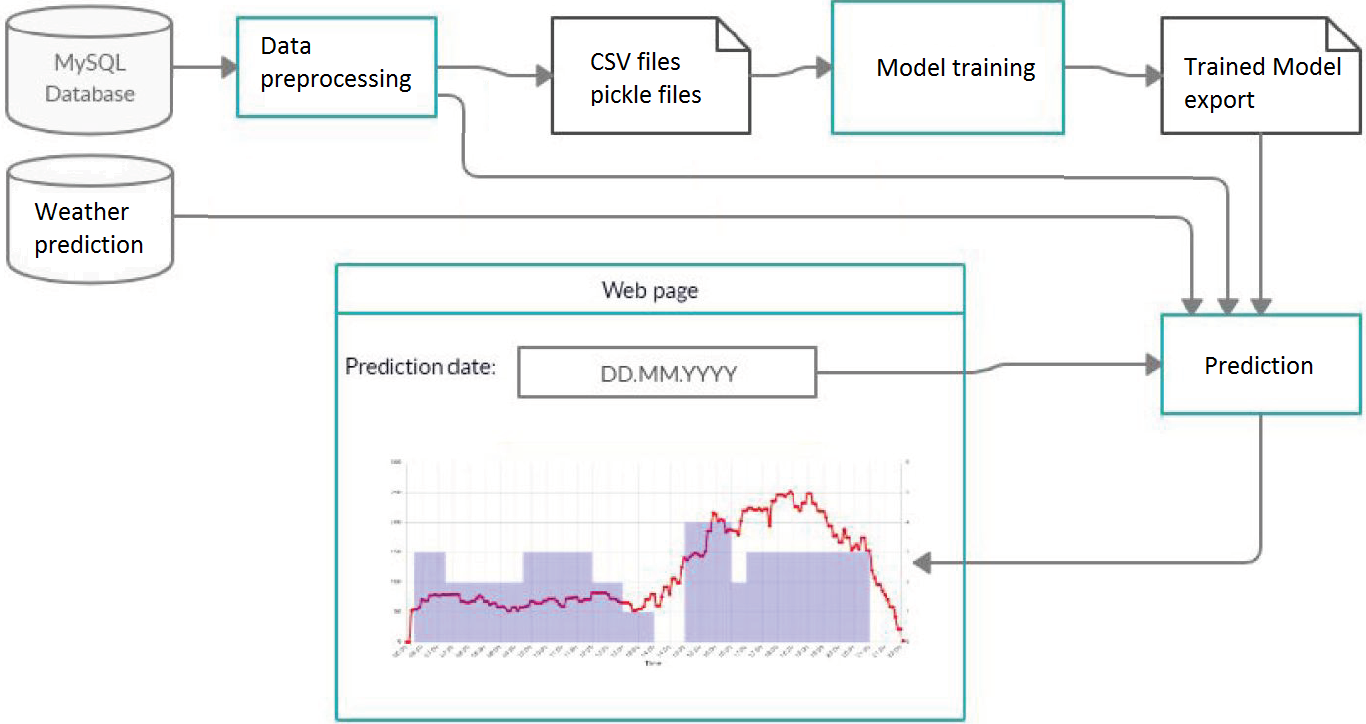
\includegraphics[width=12cm]{imgs/project_pipeline}
\caption{Diagram of project pipeline}
\label{fig:diagram_pipeline}
\end{figure}

\subsection{Metrics} \label{sec:metrics}
Mean squared error is used to measure performance of prediction. Prediction output is vector of integers representing number of people in pool. Error metrics for task like this is usually either Mean Absolute Error (MAE) or Mean Square Error (MSE). Both metrics computes average of differences between ground truth values and predicted values. The main distinction between these two metrics is that MSE uses square of difference while MAE uses absotulute difference. I chose MSE as final metrics because it punishes outliers more than MAE since the error grows quadratically with distance and this forces algorithm to minimalize number of outliers. Predictions are always generated for the whole day so it makes sense to measure performance also on the whole day. 

\begin{equation}
\label{eq:mse}
MSE_{day}(y,\hat{y}) = \dfrac{1}{n} \sum^{n-1}_{i=0}(y_i-\hat{y}_i)^2
\end{equation}

Mean square error of one day's prediction is computed using Equation \ref{eq:mse} above where $y$ is vector of ground truth data (real attendance during the whole day with 5 minute sampling). $\hat{y}$ is vector of predicted attendance in the same time steps as $y$. $n$ is number of time steps for the whole day (usually 288). $y_i$ is the $i$-th sample in vector $y$. 

The performance of implemented algorithms will be measured as a mean of $MSE_{day}$ on all days in testing dataset. This metric will show which algorithm performs better overall.

\begin{equation}
\label{eq:mse_all}
MSE_{dataset} = \dfrac{1}{k} \sum^{k-1}_{day=0}MSE_{day}(y,\hat{y})
\end{equation}

Where $k$ is the number of days in dataset. $y$ is vector of ground truth data for given $day$ and $\hat{y}$ is vector of predicted attendance for given $day$.

\section{Analysis}
\subsection{Data Exploration} \label{sec:data_exploration}

Every machine learning project starts with the data gathering and analysis. Data for this project comes from several sources. The most important data input is collected on my personal webserver that stores pool occupancy every 5 minutes into the MySQL database from publicly available data on \v{S}utka pool web page. Data are collected for past 2 years which means I have more than enough data for training, validation and testing of machine learning algorithms. But there are also many other inputs that influence attendance of swimming pool and are highly valuable for predictions. One of the most important is number of reserved swimming lines with names of organisations reserving the lines. This information is also collected from publicly available data on \v{S}utka pool web page. Next important input is time of the year that is included in timestamp of each timesample, public holidays acquired from \href{https://www.officeholidays.com/countries/czech-republic}{officeholydas.com} and finally local weather acquired from archive of \href{https://www.in-pocasi.cz/archiv/}{in-pocasi.cz}. Local weather contains information about temperature, humidity, precipitation, wind strength and air pressure from multiple stations across Prague. All these information are also stored in the MySQL database. See Image \ref{fig:db_export} for the sample export from database. History weather information is collected in database but for the occupancy prediction into the future is used 5 days weather prediction from \href{https://openweathermap.org/forecast5}{OpenWeatherMap.org} that provides free predictions via REST API. Working directly with MySQL database would not be very comfortable. This is why the database was exported, preprocessed and saved to csv files and pickle files. More about preprocessing can be found in section \ref{sec:data_preprocessing}. 

\begin{figure}[h!]
\centering
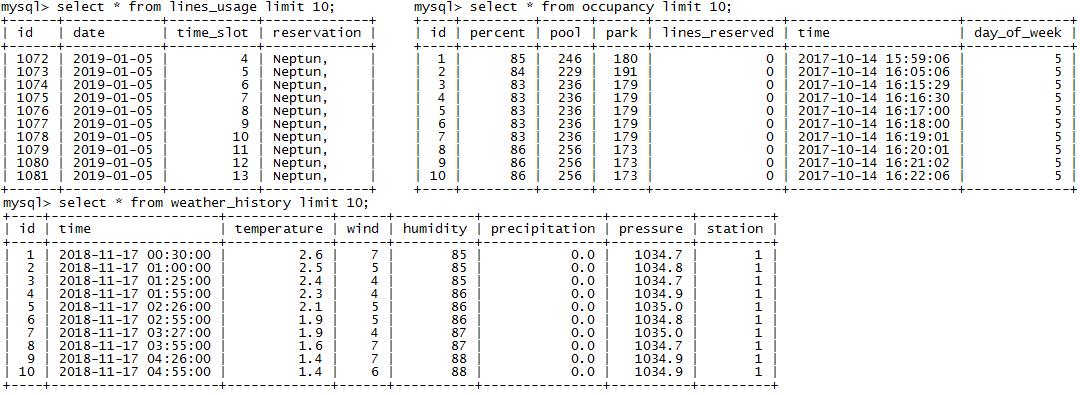
\includegraphics[width=16cm]{imgs/db_export.png}
\caption{Sample export of 10 rows from all tables in MySQL database. Top left table \emph{lines\_usage} with information about which organisation reserved line in given time. Top right table \emph{occupancy} with information about number of people in the pool. Bottom table \emph{weather\_history} with information about weather history in Prague.}
\label{fig:db_export}
\end{figure}

\subsubsection{Pool attendance data}
Attendance data are stored in table \emph{occupancy}. Data are collected every 5 minutes which results in 288 time samples from each day. As you can see on Image \ref{fig:db_export} top right there are more than just pool attendance stored for each time stamp. Following information are store in this table:
\begin{itemize}
    \item \textbf{id} - unique identifier integer of data sample.
    \item \textbf{percent} - occupancy of pool in percentage. 100 means that pool is full. 
    \item \textbf{pool} - number of people in the pool area.
    \item \textbf{park} - number of people in the park area.
    \item \textbf{lines\_reserved} - not used any more, set to 0. Number of reserved lines together with additional information are stored in table lines\_usage described in section \ref{sec:lines_usage}.
    \item \textbf{time} - timestamp with date and time.
    \item \textbf{day\_of\_week} - day of week starting with 0 for Monday.
\end{itemize}

Notice that there are number of people in pool and in park. This is because the whole \v{S}utka pool is divided into two parts. First part is pool with 50 meters swimming pool, small pool for little children, showers, two steam rooms, two saunas and resting area. Second part is park with small water park (water slides, whirlpools, outdoor relax area, foot court and bar). These two parts of the pool are connected with tourniquets so the number of people in each area is precisely monitored. Since only prediction of number of people in pool is the scope of this project columns \emph{percent} and \emph{park} are not used. Also \emph{lines\_reserved} is not used since this information is stored in separate table \emph{lines\_reserved}.

\subsubsection{Lines usage data} \label{sec:lines_usage}
Table \emph{lines\_reserved} stores information about reserved lines. Reservations can be made for 15 minutes time slots and each organisation can reserve more than one line for any number of time slots. Therefor names of the organisations and number of lines in each time slot are stored. If there is no entry for particular day or time it means that no line is reserved. Since only time slot and names of organisations that rents line in particular time slot is saved there is no information about which lines precisely are booked - only how many lines are booked. But it is not necessary to know which specific line was reserved to predict attendance, information about organisation and number of lines is sufficient. Description of table columns is following:
\begin{itemize}
    \item \textbf{id} - unique identifier integer of data sample
    \item \textbf{date} - date in format YYYY-MM-DD
    \item \textbf{time\_slot} - integer from 0 to 63 that represents time slot of swimming line reservation in reservation table on \href{https://www.sutka.eu/en/obsazenost-bazenu}{\v{S}utka swimming pool web page}
    \item \textbf{reservation} - comma separated strings containing names of clubs or organisations that rented the line. One name can be represented multiple times which means that given organisation rented multiple swimming lines
\end{itemize}

\subsubsection{Weather data}
Table \emph{weather\_history} stores historical data of weather in Prague. Data are collected from \href{https://www.in-pocasi.cz/archiv/}{in-pocasi.cz archive}.There are several measurement stations
available each with the unique id in column station. Description of table columns is following:
\begin{itemize}
    \item \textbf{id} - unique identifier integer of data sample
    \item \textbf{time} - timestamp with date and time
    \item \textbf{temperature} - temperature in degrees of Celsius
    \item \textbf{wind} - wind strength in meters per second
    \item \textbf{humidity} - humidity in percents
    \item \textbf{precipitation} - rain or snow precipitation in millimeters
    \item \textbf{pressure} - air pressure in kPa
    \item \textbf{station} - unique id of weather station where the measurement comes from
\end{itemize}

\subsubsection{Data statistics}
\begin{figure}[h!]
\centering
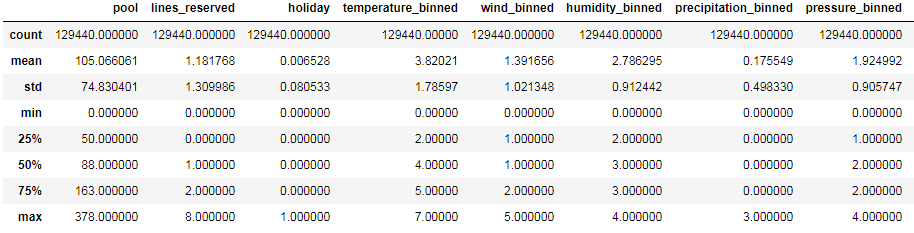
\includegraphics[width=16cm]{imgs/stats.png}
\caption{Statistics of selected data.}
\label{fig:features_stats}
\end{figure}

Image \ref{fig:features_stats} shows statistics of selected data after preprocessing. It is important to note that this means that all the data from hours when pool is closed were not used. This resulted in 129440 time samples covering 641 days. There are all available data except time stamps and also all line reservation information are represented in column \emph{lines\_reserved}. Column \emph{pool} represents attendance of pool and column \emph{holiday} represents public holidays in binary form (1 - day was public holiday, 0 - day was not public holiday). Remaining columns ending with \emph{\_binned} are weather data after preprocessing described in section \ref{sec:data_preprocessing}. From the data is visible that average attendance throughout the whole dataset at any time is 105 people with maximum attendance 378 people. There are on average 1.18 reserved lines with almost no precipitation and average temperature around bin number 4 which is from 10 to 15 degrees Celsius (more about weather data binning in section \ref{sec:bin_weather}).

\subsection{Exploratory Visualization}
\begin{figure}[h!]
\centering
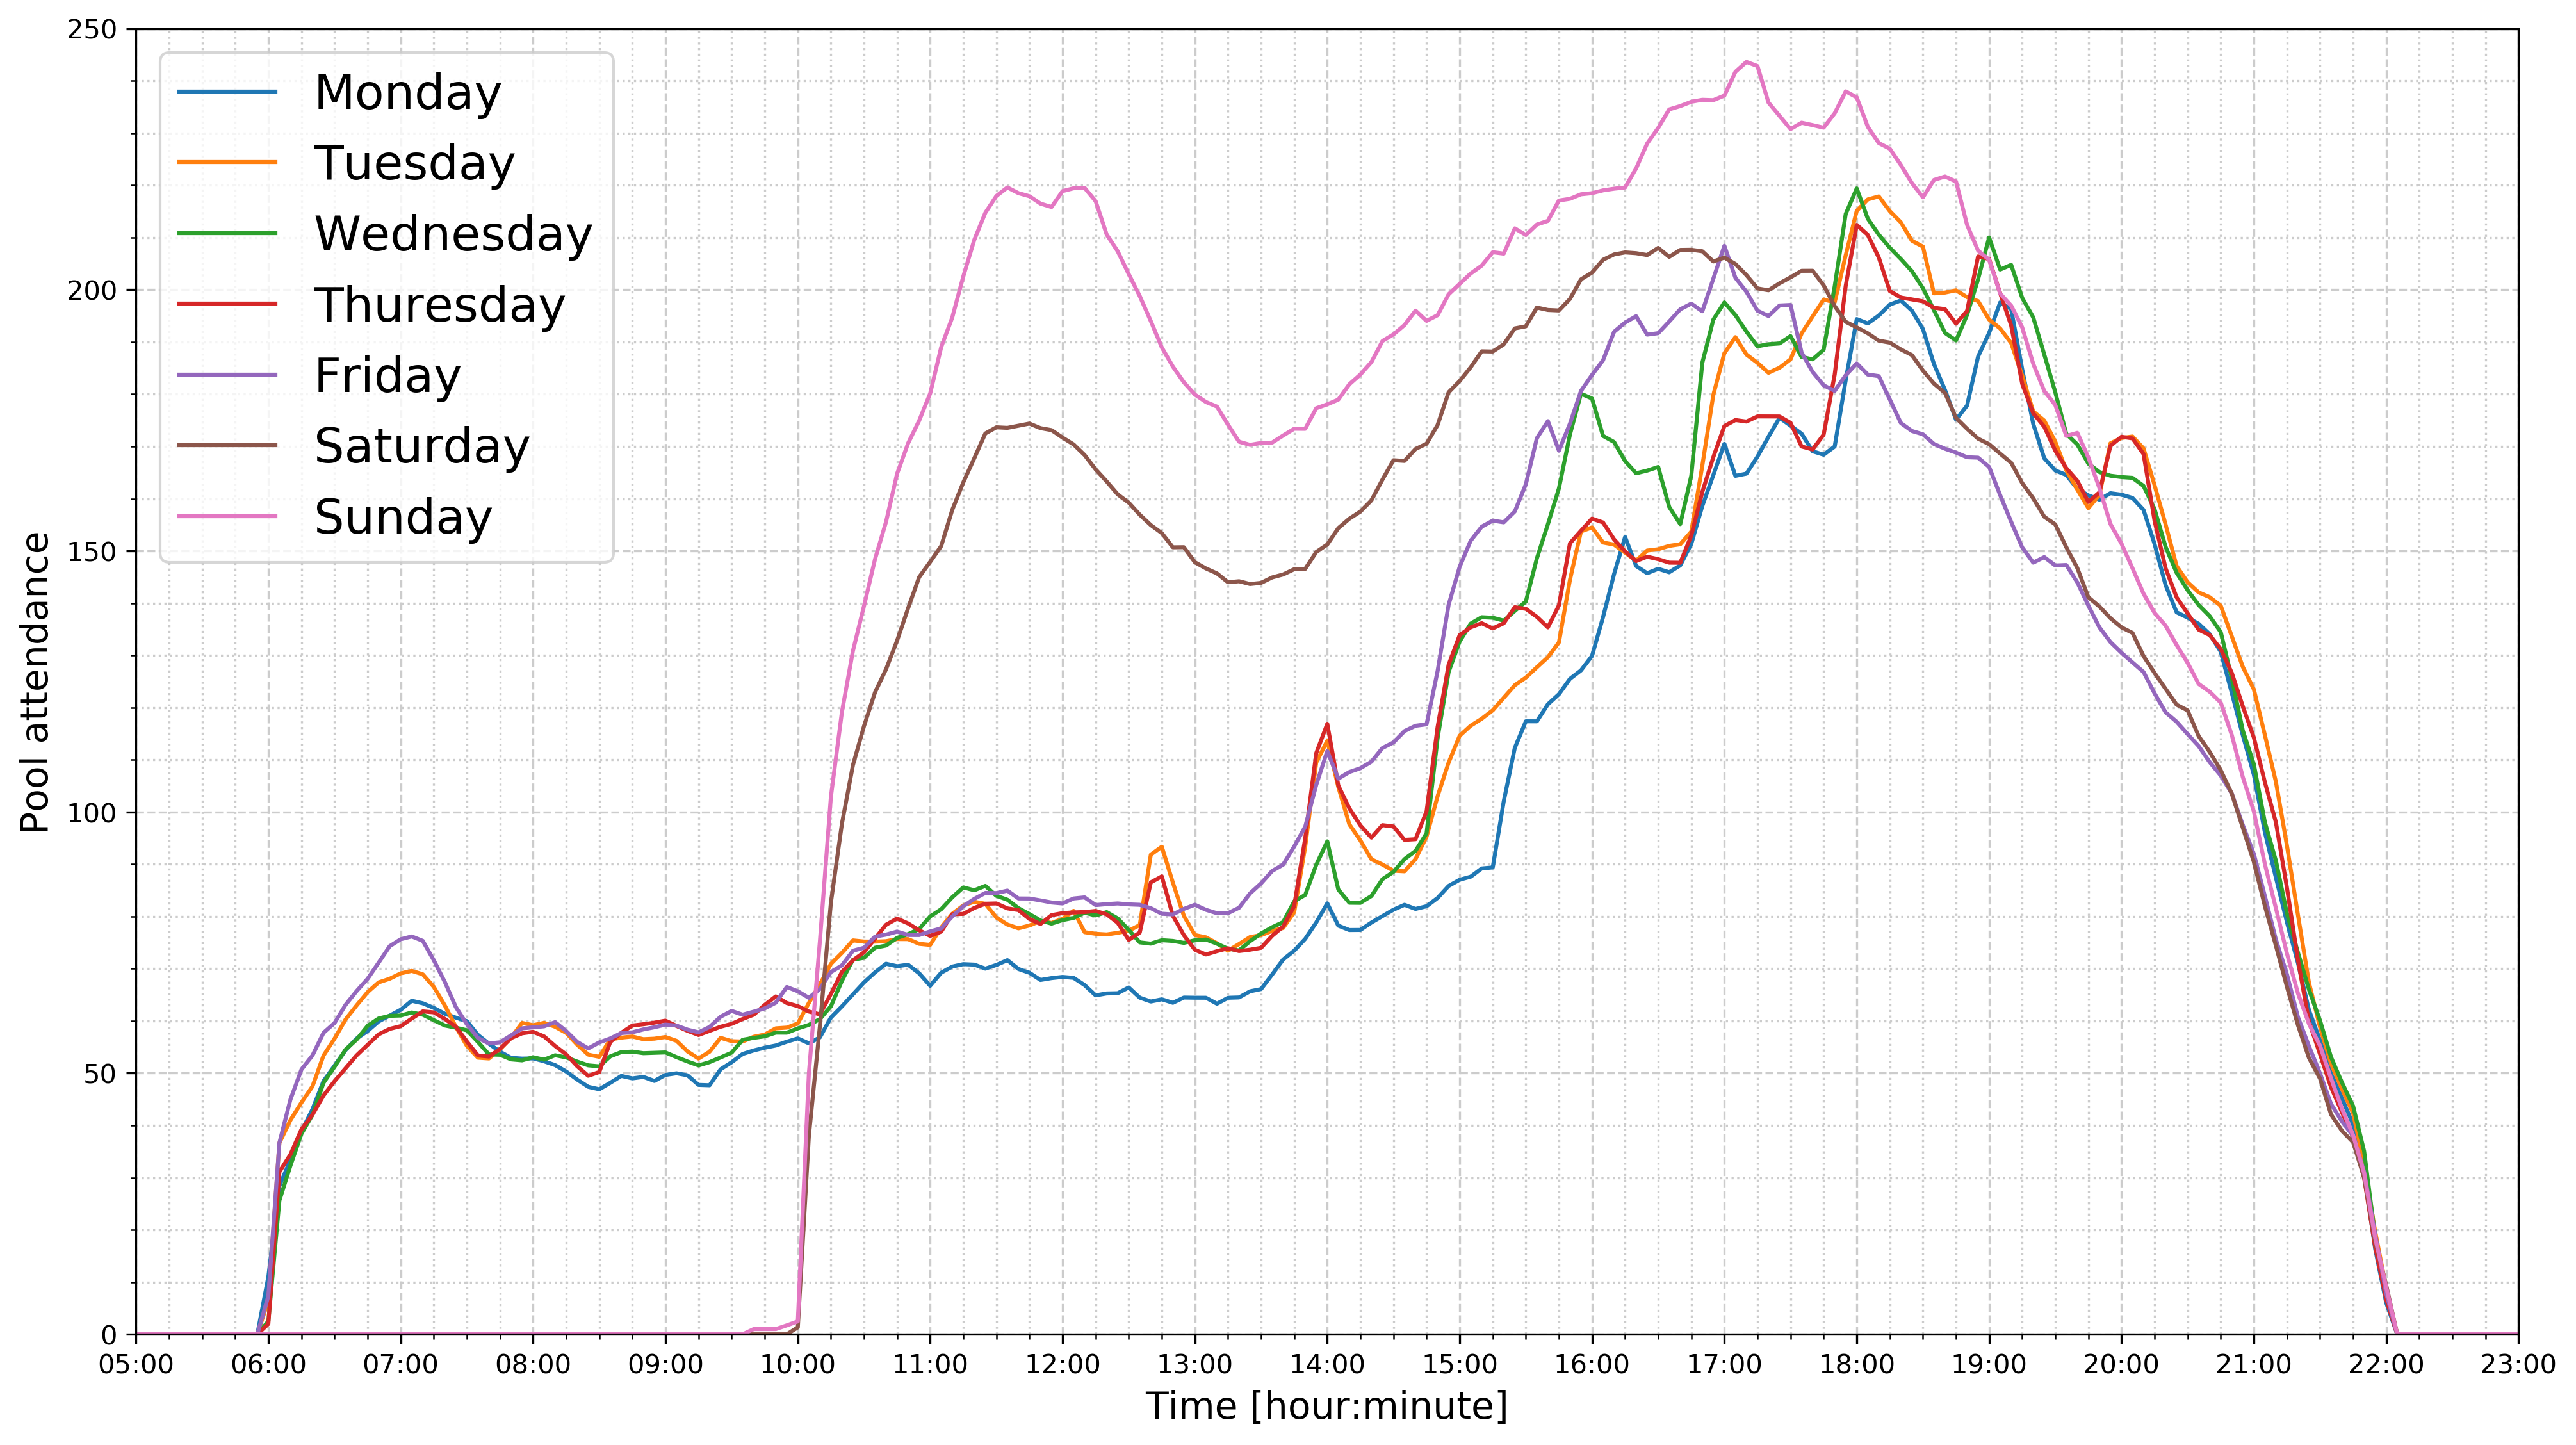
\includegraphics[width=13cm]{imgs/averages}
\caption{Average attendance for each day of week}
\label{fig:averages}
\end{figure}

Image \ref{fig:averages} shows average attendance at each day of week. This image shows several very important patterns in data. Most obvious is difference between weekend and weekday. On weekdays is pool open from 6:00 and attendance quickly rise to 50 people. Than from around 14:00 attendance rise again until 18:00 when it starts to drop until closing time at 22:00. On weekend days pool opens at 10:00 which is followed by steep increase of occupancy that drops a little around 12:00, then rise again and from 18:00 decrease until closing time at 22:00.

\begin{figure}[H]
\centering
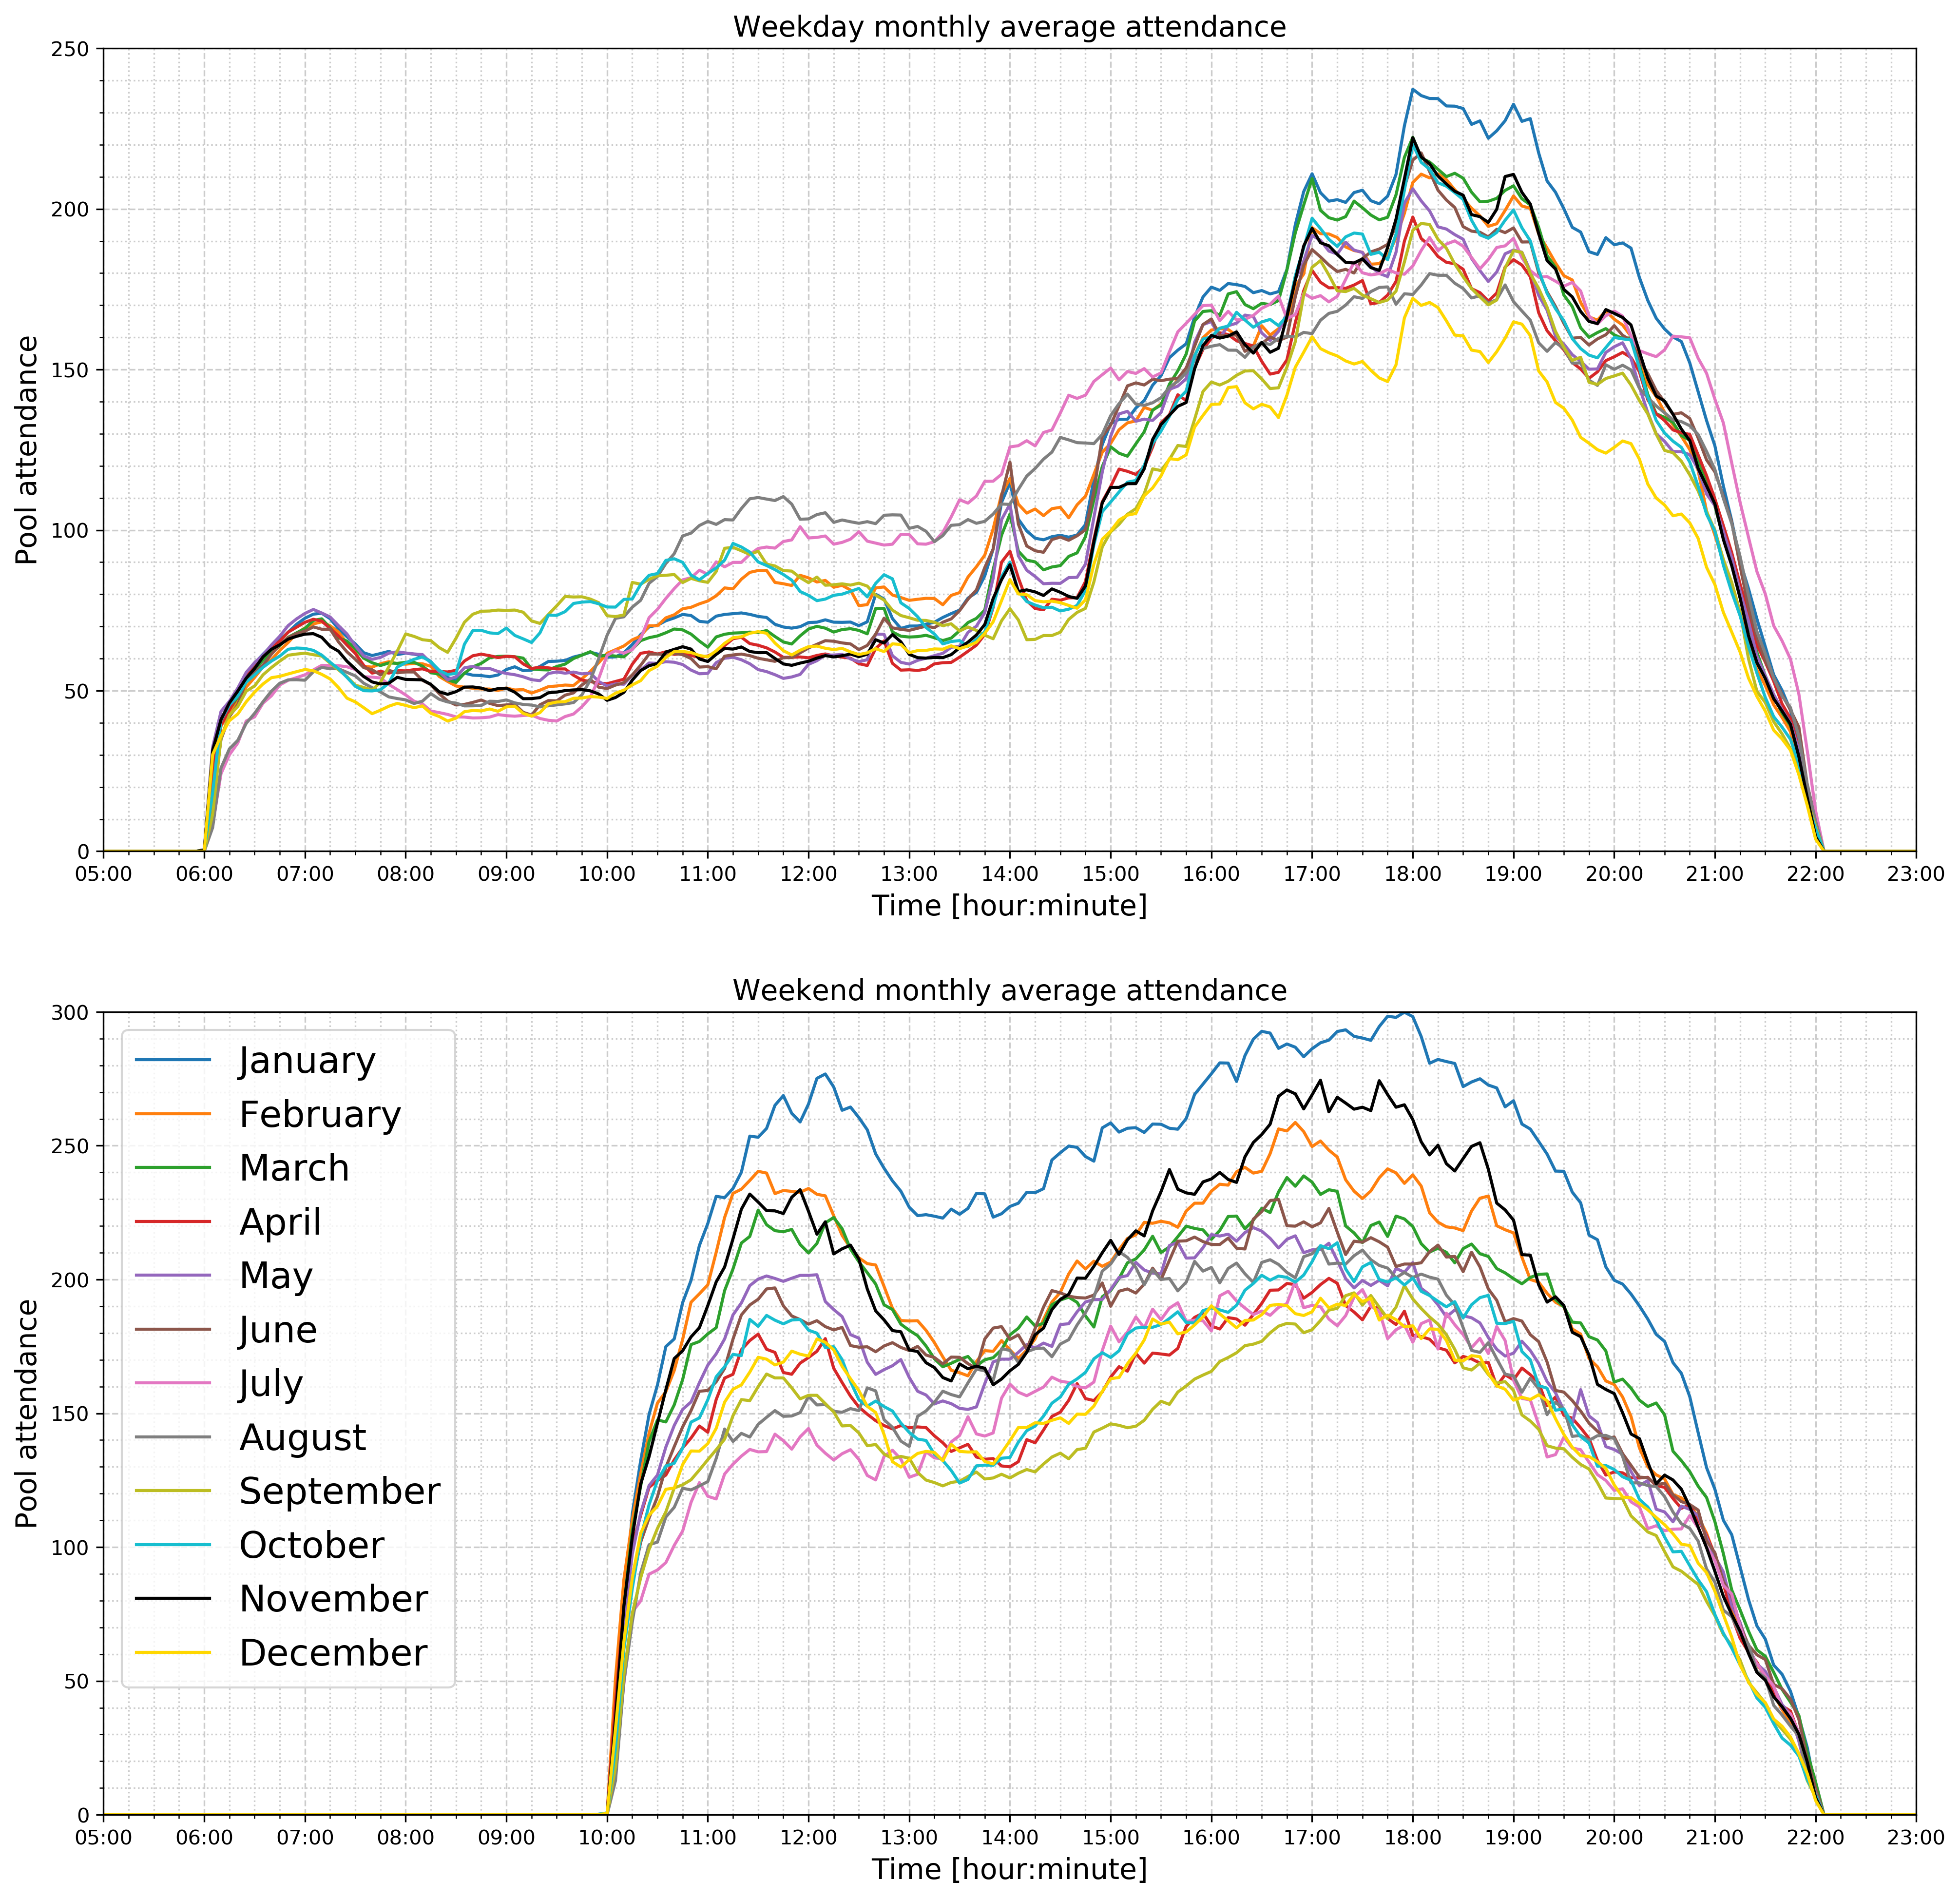
\includegraphics[width=13cm]{imgs/monthly_averages_together.png}
\caption{Monthly average attendance. Top image shows average attendance during weekdays. Bottom image shows average attendance during weekend days.}
\label{fig:monthly_averages}
\end{figure}

Image \ref{fig:monthly_averages} shows average attendance at each month at weekdays (top) and weekends (bottom). This Image shows another important pattern in data and it is the seasonality. It is interesting that weekend attendance is much more influence by seasonality than weekdays. The difference between average attendance at 18:00 in January (the busiest month) and December (the calmest month) is 70 people on weekdays but 120 on weekends. December is also interesting from another perspective. The average attendance rises from July to January with the only exception in December. This could be caused by Christmas holidays and New Year when many people have vacations, spending time with family and friend and there are also many public holidays. 

\begin{figure}[H]
\centering
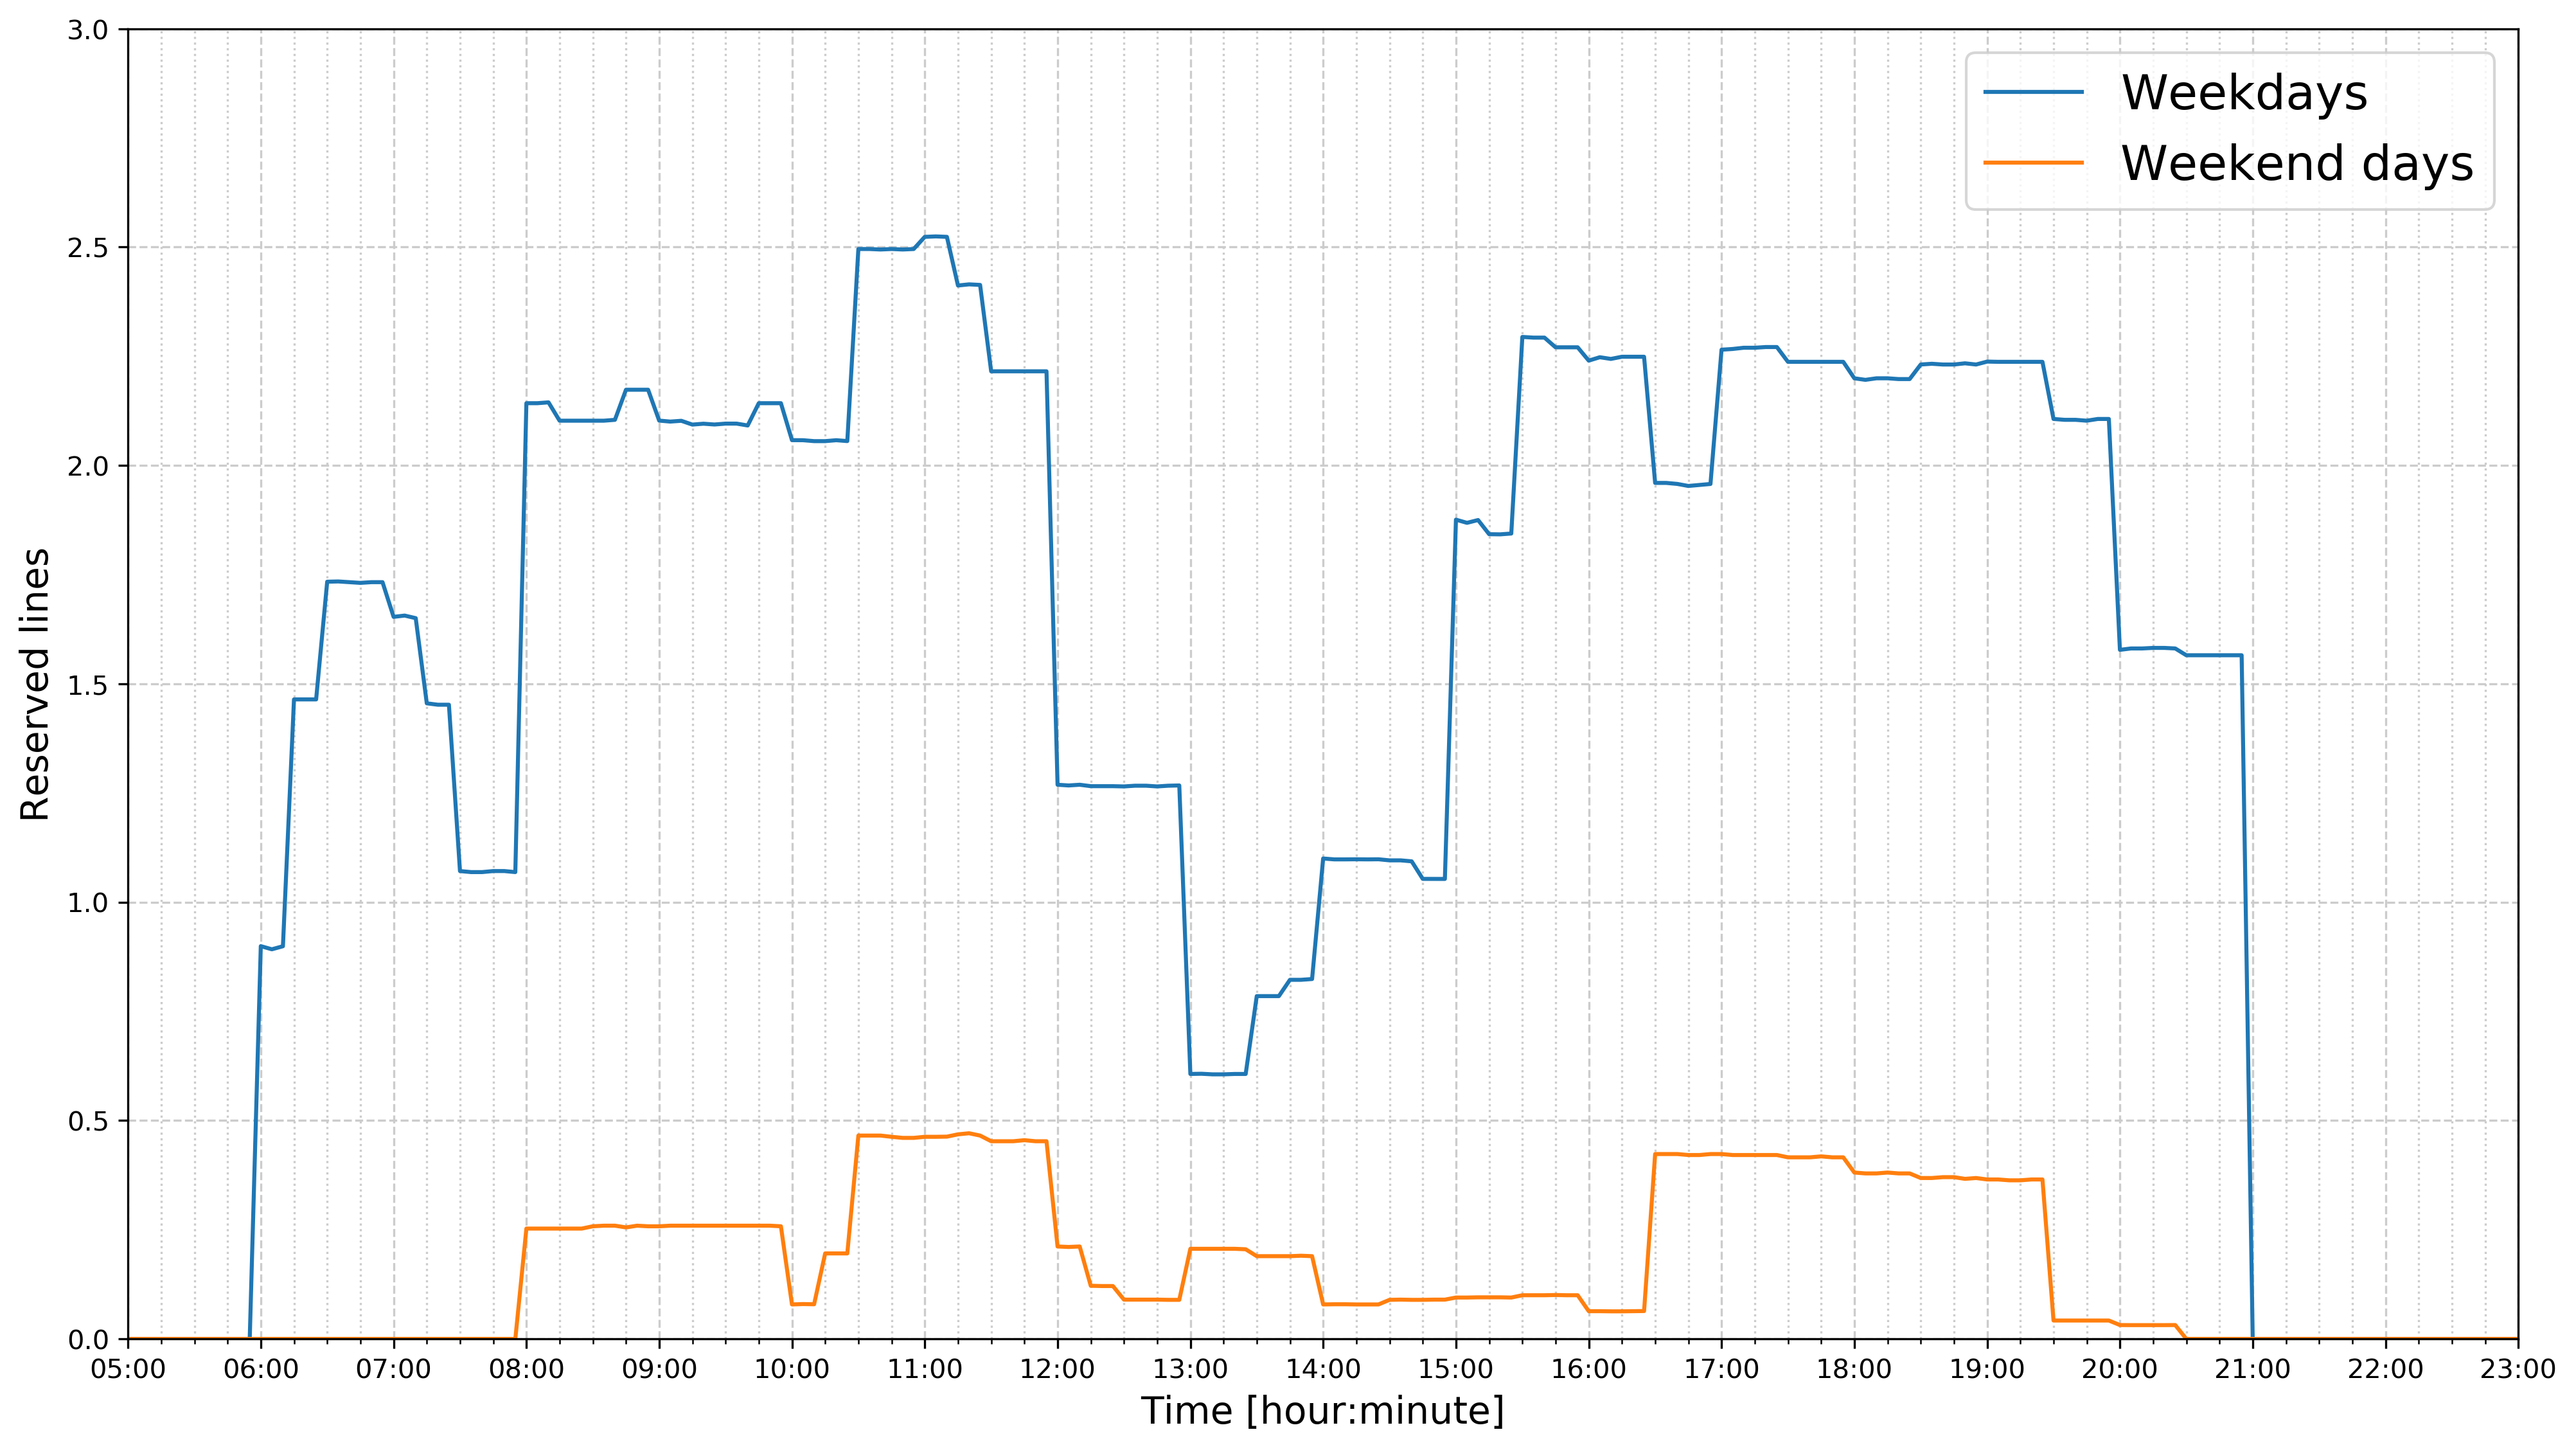
\includegraphics[width=13cm]{imgs/avg_lines.png}
\caption{Average number of reserved lines on weekdays and weekend days.}
\label{fig:lines_averages}
\end{figure}

Image \ref{fig:lines_averages} shows average number of reserved lines on weekdays and weekend days. Weekends are usually without any reservations, that is also why average number reserved lines is always under 0.5. Occupation on weekdays on the other hand are highly influence by reserved lines. There is clear pattern with over 2 lines reserved on average from 8 to 12 o'clock and than the similar pattern between 15 and 20 o'clock. This is also why I think that information about lines reservation will be important features for machine learning algorithms.

\subsection{Algorithms and Techniques}
\subsubsection{Input data}
Since all used algorithm utilizes supervised learning a sliding windows approach described in \citep{brownlee2019howtosupervised} was used to serve data. At each time stamp are all available features provided. This creates vector of input features with following content:
\begin{equation}
\label{eq:input_vector}
v(t) = (attendance(t), lines(t), minute(t), day, month, year, weather(t), org(t))
\end{equation}

Where 
\begin{itemize}
    \item $t$ is the time step of the day. Each day is sampled with 5 minute steps. So for example $t = 0$ is time 0:00, $t = 3$ is time 0:15 and $t = 287$ is time 23:55, 
    \item $v(t)$ is vector of features at time $t$.
    \item $attendance(t)$ is pool attendance at time $t$.
    \item $lines(t)$ is number of reserved lines at time $t$.
    \item $minute(t)$ is minute of the day at time $t$. Minute of the day is counted from the beginning of the day.
    \item $day$ is the day of week indexing from 0 as Monday. So for example 1 is Tuesday and 6 is Sunday.
    \item $month$ is the month of the year indexing from 0 as January. So for example 3 is April and 11 is December.
    \item $year$ is current year with offset 2015. So 4 is year 2019.
    \item $weather(t)$ is vector of weather data at time $t$. Weather data contains following in this particular order: temperature, wind, humidity, precipitation, pressure. All the weather values are binned as described in section \ref{sec:data_preprocessing}.
    \item $org(t)$ is  vector of organisations reserving swimming lines at time $t$. Precise content of this vector is described in section \ref{sec:data_preprocessing}.
\end{itemize}

Vector described above represents one time sample with all features that serves as input to prediction algorithm. Output of prediction algorithm is one integer representing predicted attendance in next time step. During the development was obvious that more input time samples then just single one produce better results. 

\subsubsection{Random Forest Classifier and Regressor}
Random Forest is an ensemble method that combines multiple decision trees. Each decision tree produces prediction and the most frequent prediction is chosen as the output of Random Forest Classifier or average of predictions for Random Forest Regressor. Randomness in name comes from random bagging during learning phase. Each decision tree is learned on different subset of training data generated by randomly sampling the training set. Also the decision at each node is made on random sub-sample of available features and the best split is used \citep{yiu2019randomforest} \citep{wiki2019randomforest}.

Random Forests have several parameters that can be tuned. Following parameters were tuned during implementation: number of trees, maximum depth of tree, minimum number of samples required to split an internal node, minimum number of samples required to be at a leaf node, number of features to consider when looking for the best split and maximum number of lead nodes. 

\subsubsection{Extra Trees Classifier and Regressor}
Extra Trees is an ensemble learning method utilizing decision trees similar to Random Forest. There are however few differences between these two classifiers. Its name is coming from extremely randomized trees and was proposed by \citep{geurts206extratree}. The main difference between Extra Trees and Random Forest is that Extra Trees does not bootstrap observations and splits node randomly. This means that randomness does not come from random data bootstrapping but from random splits of observations \citep{bhandari2019extratree}. Same parameters as for Random Forest are tuned for Extra Trees.

\subsubsection{Convolutional Neural Network}
Convolutional Neural Network (CNN) is a Deep Learning algorithm utilizing convolution mathematical operations. CNN's are most commonly used for computer vision problems but they can be used also for time series forecasting \citep{brownlee2019cnn} \citep{granat2020cnn}. Working with neural network is little different than working with standard machine learning algorithms like previously discussed Random Forest and Extra Trees. Biggest difference is need to define network structure. This was probably most time consuming task since every change of architecture requires new training that take a lot of time. Nevertheless CNN that produces satisfactory results was implemented and trained. More about this in section \ref{sec:cnn_implementation}. 

\subsubsection{Long Short-Term Memory}
Long Short-Term Memory (LSTM) are type of recurrent neural network that contains feedback memory loops. Thanks to that they can better understand sequential data such as time series like in this project. A common LSTM unit is composed of a cell, an input gate, an output gate and a forget gate. The cell remembers values over arbitrary time intervals and the three gates regulate the flow of information into and out of the cell \citep{wiki2020lstm}. 

\subsection{Benchmark}
Just by looking at the Image \ref{fig:averages} we can clearly see that average attendance progress throughout all weekdays looks similar. Same is true for weekend days. On the other hand looking at Image \ref{fig:monthly_averages} we can definitely see seasonality trends in each month. For example January afternoon attendance is more 100 people larger than September attendance. This is why I chose monthly average (one for weekdays and one for weekend days) to be the benchmark prediction model. It provides reasonable good approximation of real attendance throughout the month since it usually does not change a lot during one month. 

On the other hand, when comparing each day individually some minor differences during the day's progress that may be caused by weather, line reservations, public holidays or some other features are visible. This is the potential for machine learning algorithms to be able to spot these minor differences and utilize these features to provide more accurate predictions than simple monthly average.

\subsubsection{Monthly average} \label{sec:monthly_average}
For each time stamp throughout the day is computed average attendance at given month. Since the attendance on weekdays and weekends differs highly (see Image \ref{fig:averages}) two average predictions are generated for each month - one for weekdays and one for weekend days. 

\begin{equation}
\label{eq:monthly_avg}
\hat{y}_i = \dfrac{1}{m} \sum^{m-1}_{j=0}y_j
\end{equation}

Where $\hat{y}_i$ is prediction at time stamp $i$. $m$ is number of time samples in training set for predicted month in given week time (weekday or weekend).

\section{Methodology}
\subsection{Data Preprocessing} \label{sec:data_preprocessing}
Origin of data and it's structure in MySQL database is described in previous section \ref{sec:data_exploration}. In this section are more in depth discussed preprocessing steps to make data easily accessible for machine learning algorithms fitting and predictions.

First part of preprocessing was to convert data from MySQL database to csv file. Code for all preprocessing tasks can be found in file \emph{preprocessing\_data.py}. Database contains three tables with information about attendance, swimming pool lines reservation and weather. As mentioned in \ref{sec:problem_statement} public holidays should be also used but are not present in database. Public holiday dates for all years in dataset were downloaded from \href{https://www.officeholidays.com/countries/czech-republic}{officeholydas.com}. For the export I decided to use structure of table \emph{occupancy} where each row represents one time stamp every 5 minutes. To each time stamp is than exported number of reserved lines and which organisations are reserving lines, all weather information from table \emph{weather\_history} at measurement station closest to the pool and flag if this day is public holiday or not. Result of this preprocessing using Pandas is Data Frame with following structure:

\begin{figure}[h!]
\centering
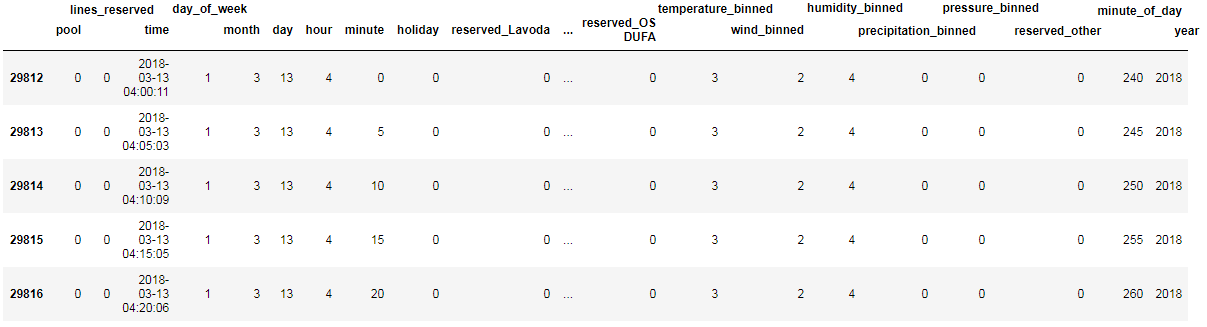
\includegraphics[width=16cm]{imgs/dataframe_head}
\caption{Structure of Data Frame after initial preprocessing and refinement that connects all available data into one table.}
\label{fig:dataframe_structure}
\end{figure}

You can see on Image \ref{fig:dataframe_structure} that only information used from \emph{occupancy} table is time stamp and pool attendance. Other data are not relevant for the occupancy of swimming pool itself. Another preprocessing step visible on Image \ref{fig:dataframe_structure} is reshaping of organisations reservation data. Database table \emph{lines\_usage} store names of organisation reserving lines in comma separated string while in this Data Frame have each organisation it's own column and value on each row represents number of lines reserved by given organisation in time stamp at that row. 

Next preprocessing step was to split all data into \emph{Days} (you can find class Day in \emph{utils.py}). \emph{Day} is a class containing DataFrame with feature vectors only for one day starting one hour before opening and ending one hour after closing time of the pool. This class also contains several methods for easy access of data and other data transformation like normalization. It is important that data for neural networks are normalized otherwise neural network methods can have problems properly learn. All 641 \emph{Days} are stored pickle split into training, testing and validation set with approximate proportions 2:2:1 which means 263 training days, 248 testing days and 130 validation days. These are not in exact 2:2:1 proportion because of another preprocessing step that was removing days with missing data. Few days had missing measurements and since it was just the small number of days I decided to remove all days with missing data completely from dataset.

\subsection{Implementation}
\subsubsection{Random state}
One of the most important task during implementation was to make sure that all the computations and learning task are reproducible. Since many steps in project pipeline involves randomness it is necessary to make sure that all random operations use the same random seed and therefore can be reproduced. Throughout the whole project was used random seed 17 for all Numpy, scikit learn, keras and tensorflow computations.

\subsubsection{Helper classes}
Several helper classes were implemented to make the work with data and algorithms easier. They are:
\begin{itemize}
    \item \textbf{Days} - \emph{utils.py} - class holding data for one day and providing several getters for the data like: whole day data, whole day normalized data or building time series for N time steps	        	\item \textbf{WeatherData} - \emph{utils.py} - helps during preprocessing to handle weather data from multiple measuring stations
    \item \textbf{DaysStatistics} - \emph{days\_statistics.py} - computes average attendance for each month and day. Highly used for benchmark model Monthly Average
    \item \textbf{DataHelper} - \emph{data\_helper.py} - most used class throughout the whole implementation. Contains helper methods to measure error of predictor, regenerate data in desired format, holds all data vectors or plot predictions
\end{itemize}

\subsubsection{Monthly Average}
Benchmark model Monthly Average was implemented according to description in section \ref{sec:monthly_average} and code can be found in file \emph{models/monthly\_average.py}. Averages for whole day at 5 minute steps were computed for each month with distinction for weekdays and weekend days. Computed averages were saved to pickle.
 
\subsubsection{Random Forest and Extra Tree algorithms}
In total four algorithms that are build on decision trees were implemented. They are Random Forest Classifier, Random Forest Regressor, Extra Trees Classifier and Extra Trees Regressor. Since output of prediction in this project is integer representing number of people in pool it can be viewed as a regression task and using classifiers seems as wrong choice. Nevertheless I wanted to compare how would classifiers perform against regressors on this task. All four algorithms were used from Scikit learn Machine Learning python library in version 0.20. This library makes implementation very easy. Preprocessed data are served info \emph{fit} function that handles all learning tasks and fitted algorithm is than ready to be used for predictions. It is however necessary to setup algorithms with parameters best suited for the task. Since there are many parameters to tune it is best to use automated tuning tool such as scikit learn's Grid Search. You can define range of parameters you would like to use, Grid search algorithm tests all possible combinations and returns fitted algorithm with the best parameters for the job. 

Searching for the best parameters turns out to be much more complicated than expected. The biggest problem is that Grid searching algorithm measures error on predictions made always only one step into the future. But the goal of this project is to generate predictions for the whole day. In order to overcome this issue was necessary to develop grid search algorithm better suited to needs of this project. You can read about my implementation of grid search in section \ref{sec:my_grid_search}. 


\subsubsection{Neural Network algorithms} \label{sec:cnn_implementation}
Convolution Neural Network (CNN) and Long short-term memory (LSTM) neural networks were implemented. For the implementation was used Keras 2.3.1 with Tensorflow 2.0 backend. Throughout the implementation were tested many different architectures with many parameter settings mostly inspired by \citep{brownlee2019cnn} and \citep{brownlee2019lstm}. In the end it appears that very deep networks were unnecessary overhead for task like this and more shallow networks produced better results in much shorter time. You can see final architectures on Images \ref{fig:cnn} and \ref{fig:lstm}.

\begin{figure}[h!]
\centering
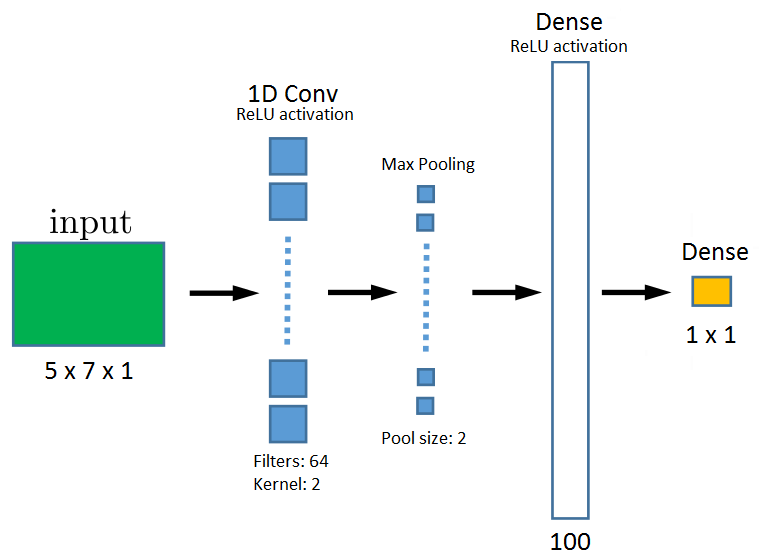
\includegraphics[width=10cm]{imgs/cnn}
\caption{Convolutional Neural Network architecture}
\label{fig:cnn}
\end{figure}

\begin{figure}[h!]
\centering
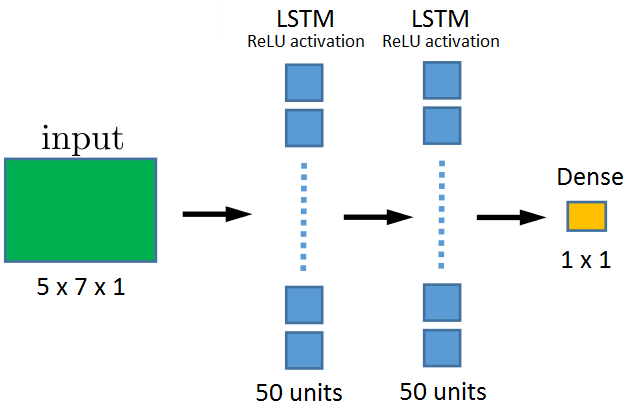
\includegraphics[width=8cm]{imgs/lstm.png}
\caption{Long Short Term Memory Network architecture}
\label{fig:lstm}
\end{figure}

To make implementation, parameter tuning and especially testing different architectures easier, neural network base class was implemented. NeuralNetworkBase class (\emph{models/neural\_network\_base.py}) is abstract base class for both LSTM (\emph{models/lstm.py}) and CNN (\emph{models/cnn.py}) algorithm implementation. It implements methods used by both networks such as fitting, loading and saving of model or computation of mean square error on whole dataset. The only abstract method necessary to implement by derived classes is \emph{build\_model} where the architecture of network is defined. This way I was able to make classes with many versions of neural networks but only by inheriting NeuralNetworkBase and implementing abstract \emph{build\_model} method.

\subsubsection{Web application}
Once the machine algorithms were train it was time to deploy them to live web page. Simple web page was made with charts showing live occupancy of pool together with predictions for the whole day. You can see screenshot of web page on Image \ref{fig:web} or visit the live web page on address: \href{http://80.211.145.114/}{http://80.211.145.114/}.

\begin{figure}[h!]
\centering
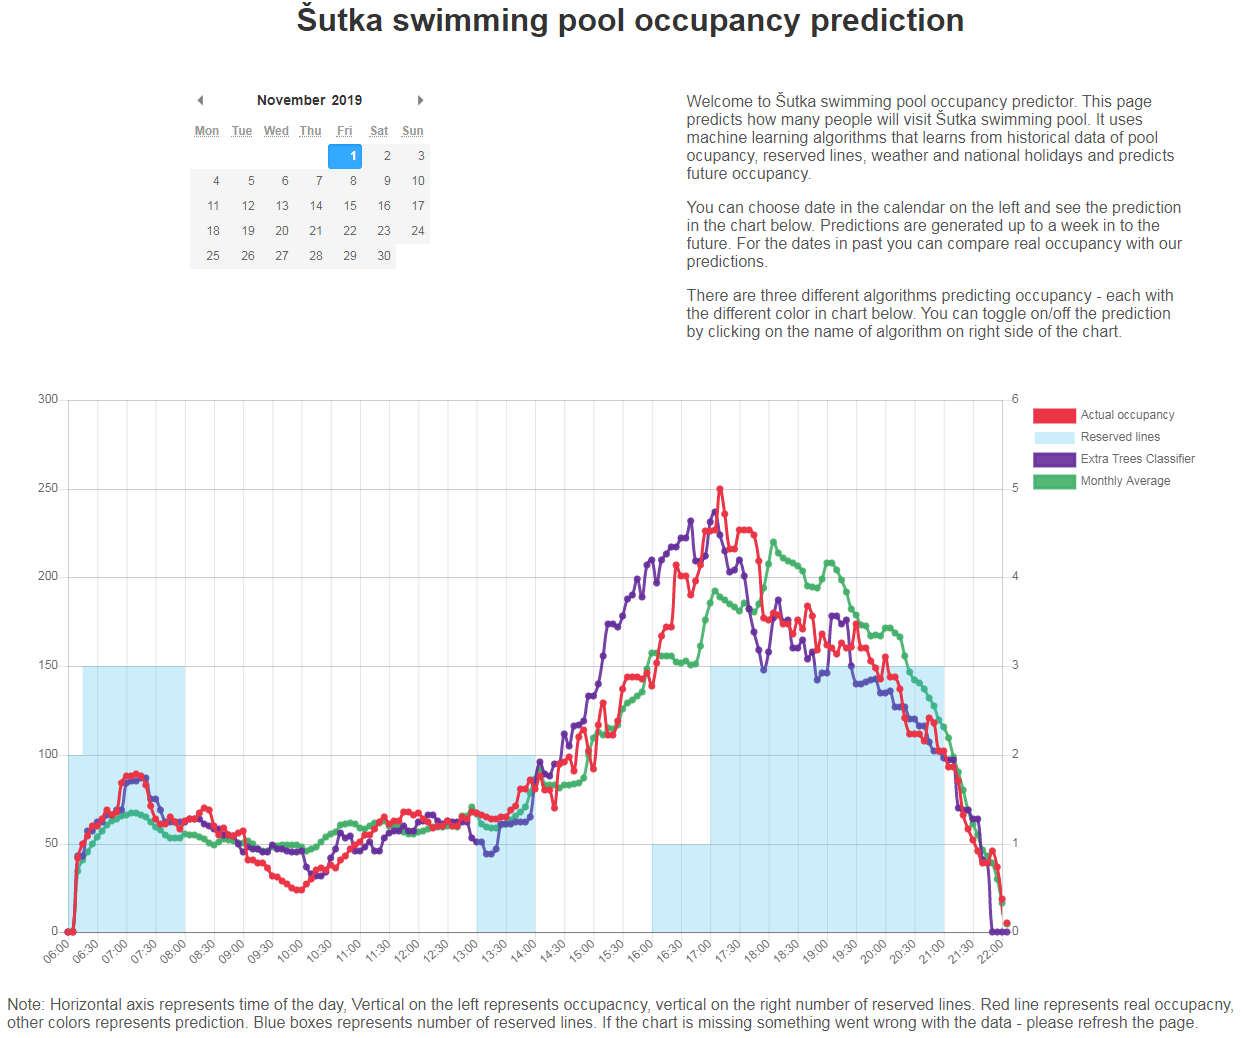
\includegraphics[width=12cm]{imgs/webpage.png}
\caption{Web page with predictions.}
\label{fig:web}
\end{figure}

Web page features calendar where visitors can pick a day (using \href{https://github.com/Pikaday/Pikaday}{Pikaday} JavaScript library) from past to see how good were the predictions in the past or select few days into the future to see future predictions. All the data are visualized in chart where visitors can enable/disable each predictions. Whole web page is one static HTML page with single JavaScript script that generates charts using \href{https://www.chartjs.org/}{ChartsJS} library from precomputed CSV files. CSV files with predictions are generated each day at midnight. CSV files generation is triggered by a cron job on the webserver that is also hosting the web page. Cron job executes python script that is using pretrained models described above. You can find all the code for web page and webserver in folder \emph{web}.

\subsection{Refinement}
\subsubsection{Bin weather data} \label{sec:bin_weather}
Weather data presented large spectre of values but initial tests on Random Forests and LSTMs shows that this data had very little information gain and increase size of Random Forest and training time of LSTMs. That is why I decide to bin weather data to following bins:
\begin{itemize}
    \item temperature - temperature in degrees of Celsius to following 8 bins:
    
    $(-100, -5], (-5,0], (0,5], (5,10], (10,15], (15,20], (20,25], (25, 100]$
    \item wind - strength in meters per second to following 6 bins:
    
    $(-1,1], (1,5], (5,10], (10,15], (15,20], (20, 1000]$
    \item humidity - humidity in percent to following 5 bins: 
    
    $(-1,20], (20,40], (40,60], (60,80], (80,100]$
    \item precipitation - rain or snow precipitation in millimetres to following 4 bins: 
    
    $(-1.0,0.1], (0.1,5.0], (5.0,10.0], (10.0,1000.0]$
    \item pressure - air pressure in kPa to following 5 bins: 
    
    $(0,1000], (1000,1010], (1010,1020], (1020,1030], (1030,2000]$
\end{itemize}

Unfortunately even after this refinement weather data still brings little to no performance gain and both neural network algorithms performed even better without the weather data. 

\subsubsection{Remove organisations with few reservations}
Encoding each organisation as new column in Data Frame with all features generated more than 100 extra columns for more than 100 organisations. But many organisations had just very few reservations and would not be beneficial to keep this information in Data Frame. That is why only organisations that regularly reserve lines and therefore their reservation could have significant influence of overall attendance were kept in Data Frame. All the other organisations (with less than 200 reservation in total) were compressed into one column \emph{reserved\_other}. This led to reduction of number of columns to reasonable 42. 
This change significantly reduced dimensionality of data improved learning speed and reduced size of fitted models. 

\subsection{Limit output of prediction to 0 - 400 interval}
As mentioned before the prediction for whole day is generated by using output of one prediction as input to prediction for the next step. In some situations the Neural Network algorithms increase/decrease predicted number in each step up to impossible high/low values. Limit for the output of algorithm was introduced that keeps predictions between 0 and 400 to prevent this behaviour. These number seems legit since maximal number of visitors in data set is 378. This helps to drop MSE of neural network algorithms to reasonable values since under some special conditions they can produce highly wrong predictions that would lead to enormously high MSE.

\subsection{Implementation of my own grid search} \label{sec:my_grid_search}
Regular grid search is computing MSE on prediction one time sample into the future. Since the change in attendance during one time step is usually very small, this means all algorithms quickly converges close to zero error and scikit learn Grid search output was unusable. Therefore I decided to implement my own Grid search (code in \emph{grid\_search.py}) algorithm that compares models based on their performance on whole validation set day by day using metric described in section \ref{sec:metrics}. The other benefit is that since all implemented algorithms can work with one or more time steps from the history to produce prediction into the future this grid search also helps to optimize number of time steps into the past used as input for the model. This grid search algorithm helped to find best parameters for all Extra Trees and Random Forest algorithms improving their performance up to 30\% from scikit learn Grid search.

\section{Results}
\subsection{Model Evaluation and Validation}
Six models plus one benchmark model were implemented and trained. All models were evaluated using testing dataset containing 248 days. Each model generated prediction for all days in dataset and their mean squared error was compared. You can see the results on Image \ref{fig:all_models_result}  

\begin{figure}[h!]
\centering
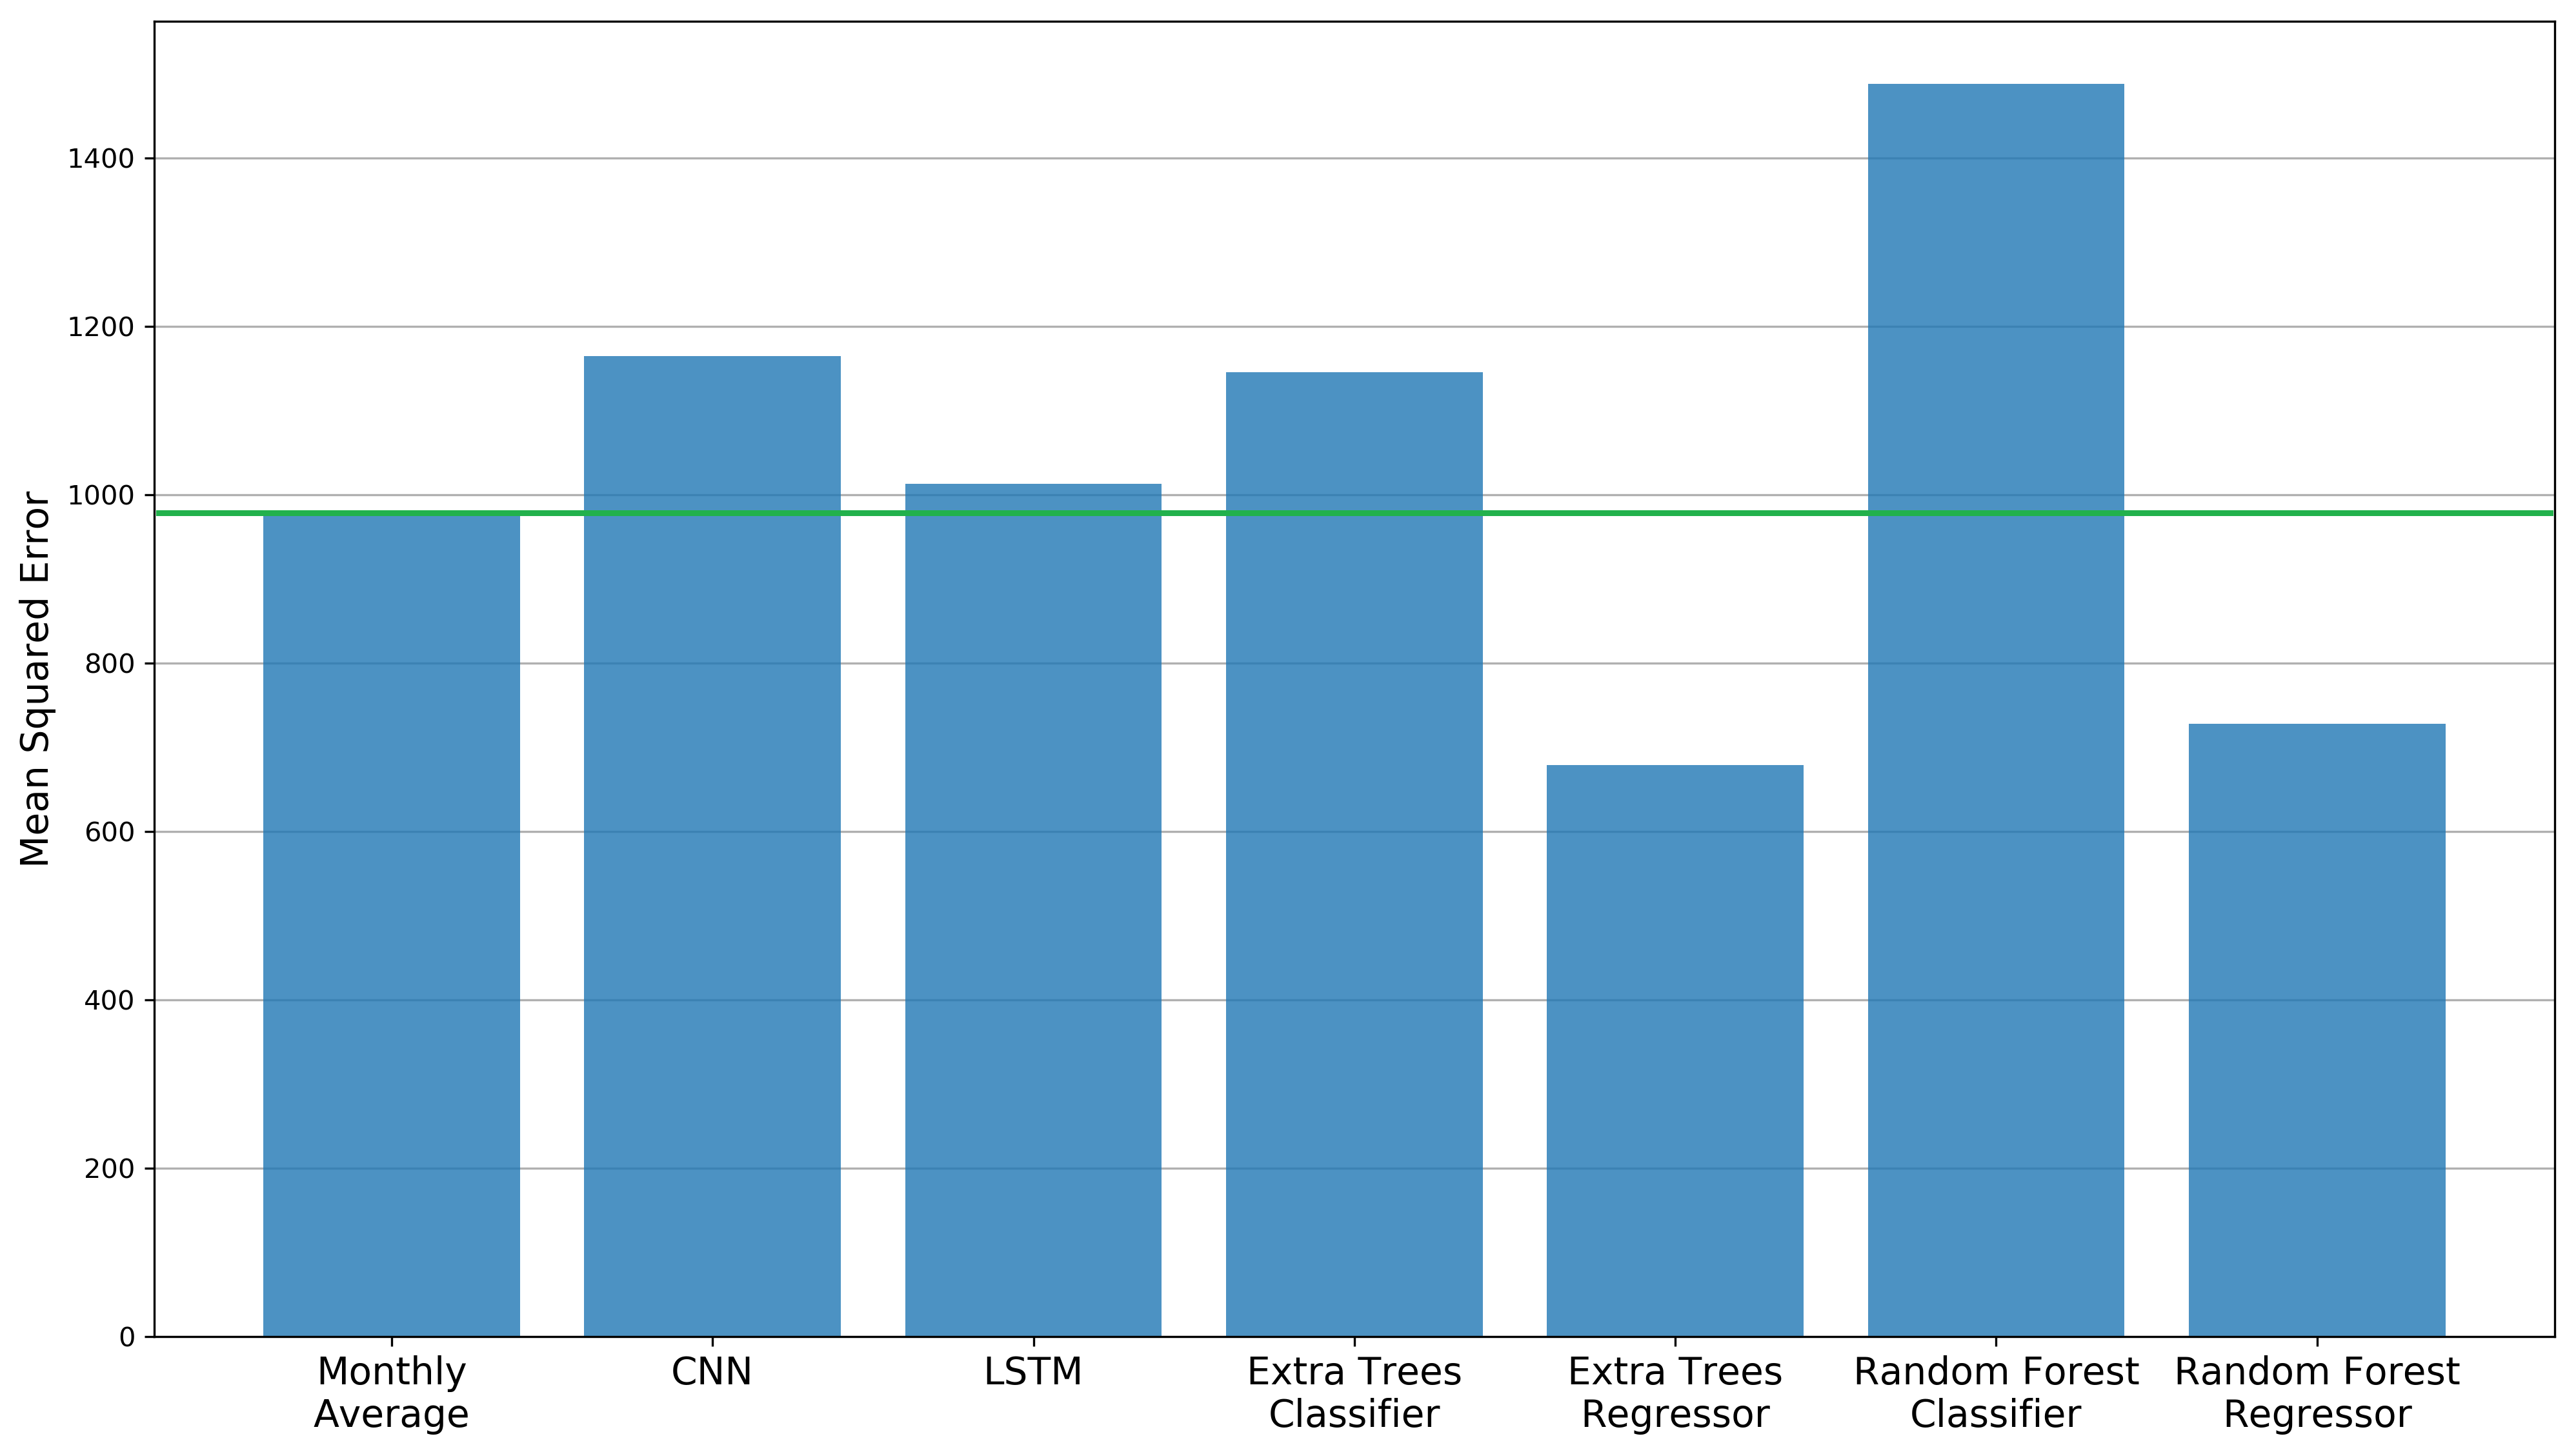
\includegraphics[width=16cm]{imgs/performance.png}
\caption{Mean Squared Errors of all implemented models. Green line shows performance of benchmark model.}
\label{fig:all_models_result}
\end{figure}

You can see that performance of simple Monthly Average benchmark model is very good with \textbf{MSE 979}. In fact beating this performance turns out to be quite the challenge. Disappointment was performance of neural networks. It was very difficult to produce some reasonable performance from both models. CNN model turns out to be the worse. After testing several different architectures and different number of input time steps the best model performs still poorly with \textbf{MSE 1488}. LSTM performance was much better than CNN's but still not good enough for benchmark model. LSTM's best performance is \textbf{MSE 1013}. Little better performance than CNN produced Extra Trees Classifier. Even thou I did not expect very good results from both classifiers, Extra Trees produced satisfactory results with \textbf{MSE 1146}. Random Forest Classifier was performance was the worst of all tried models with \textbf{MSE 1488}. It is worth mentioning that little better performance was possible to achieve using classifiers with higher number of trees (with MSE around 1000 for Extra Trees). The problem was that from around 50 trees the classifiers become so large that even my 32GB RAM was too small for them and pickle with the model was larger than 20GB. Best performances produced Extra Trees Regressor and Random Forest Regressor. It was expected that both will preform much better than both classifiers but little unexpected that they will perform even better than neural networks. Random Forest Regressor reached \textbf{MSE 728} a the best performance overall produced Extra Trees Regressor with \textbf{MSE 659}.

\begin{figure}[h!]
\centering

\includegraphics[width=16cm]{imgs/placeholder.png}
\caption{Results of Extra Trees Regressor on new data.}
\label{fig:new_data}
\end{figure}

Image \ref{fig:new_data} shows how Extra Trees Regressor handles new data. Dataset for this project was taken from November 2017 to November 2019. On this image you can se results from December 2019 and January 2020. There are several great prediction almost precisely predicting the whole day (WRITE WHICH IMAGES IS IT) but on the other hand several images where Extra Trees Regressor struggles. This is mostly due to new patter introduced during October 2019. During weekdeys morning several school swimming courses occur which results with very high and very steep increase of attendance from usual average of around 50 up to 200 or even 400. Since there are very little training data for this situation all models have troubles reacting to it. On the other hand it should be possible to fit model that will learn this behavior once there is enough training data. Especially since this happens with line reservation from organisation \emph{Lavoda} and models should be able to recognise this patter.

\color{red}
TODOs:
\begin{itemize}
    \item influence of parameter tuning on algorithms
    \item image with MSE of all methods on testing data - bar chart
    \item image for RFC and ETC with n\_estimators on x axis and MSE on y axis
\end{itemize}
\color{black}

\subsection{Justification}
Results of both classifiers were indication of some error in approach with CNN's a possible even LSTM's. On the other hand results of both regressors were very good especially the Extra Tree Regressor. It produced more than 30\% better MSE than benchmark model which is a big success. 

\color{red}
TODOs:
\begin{itemize}
    \item Are the final results found stronger than the benchmark result reported earlier?
    \item Have you thoroughly analysed and discussed the final solution?
    \item Is the final solution significant enough to have solved the problem?
\end{itemize}
\color{black}

\section{Conclusion}

\subsection{Free-Form Visualization}
\color{red}
TODOs:
\begin{itemize}
    \item Construct conclusion about your results, and discuss whether your implementation adequately solves the problem.
    \item What was good and what bad
    \item Further improvements
\end{itemize}
\color{black}

\begin{figure}[h!]
\centering
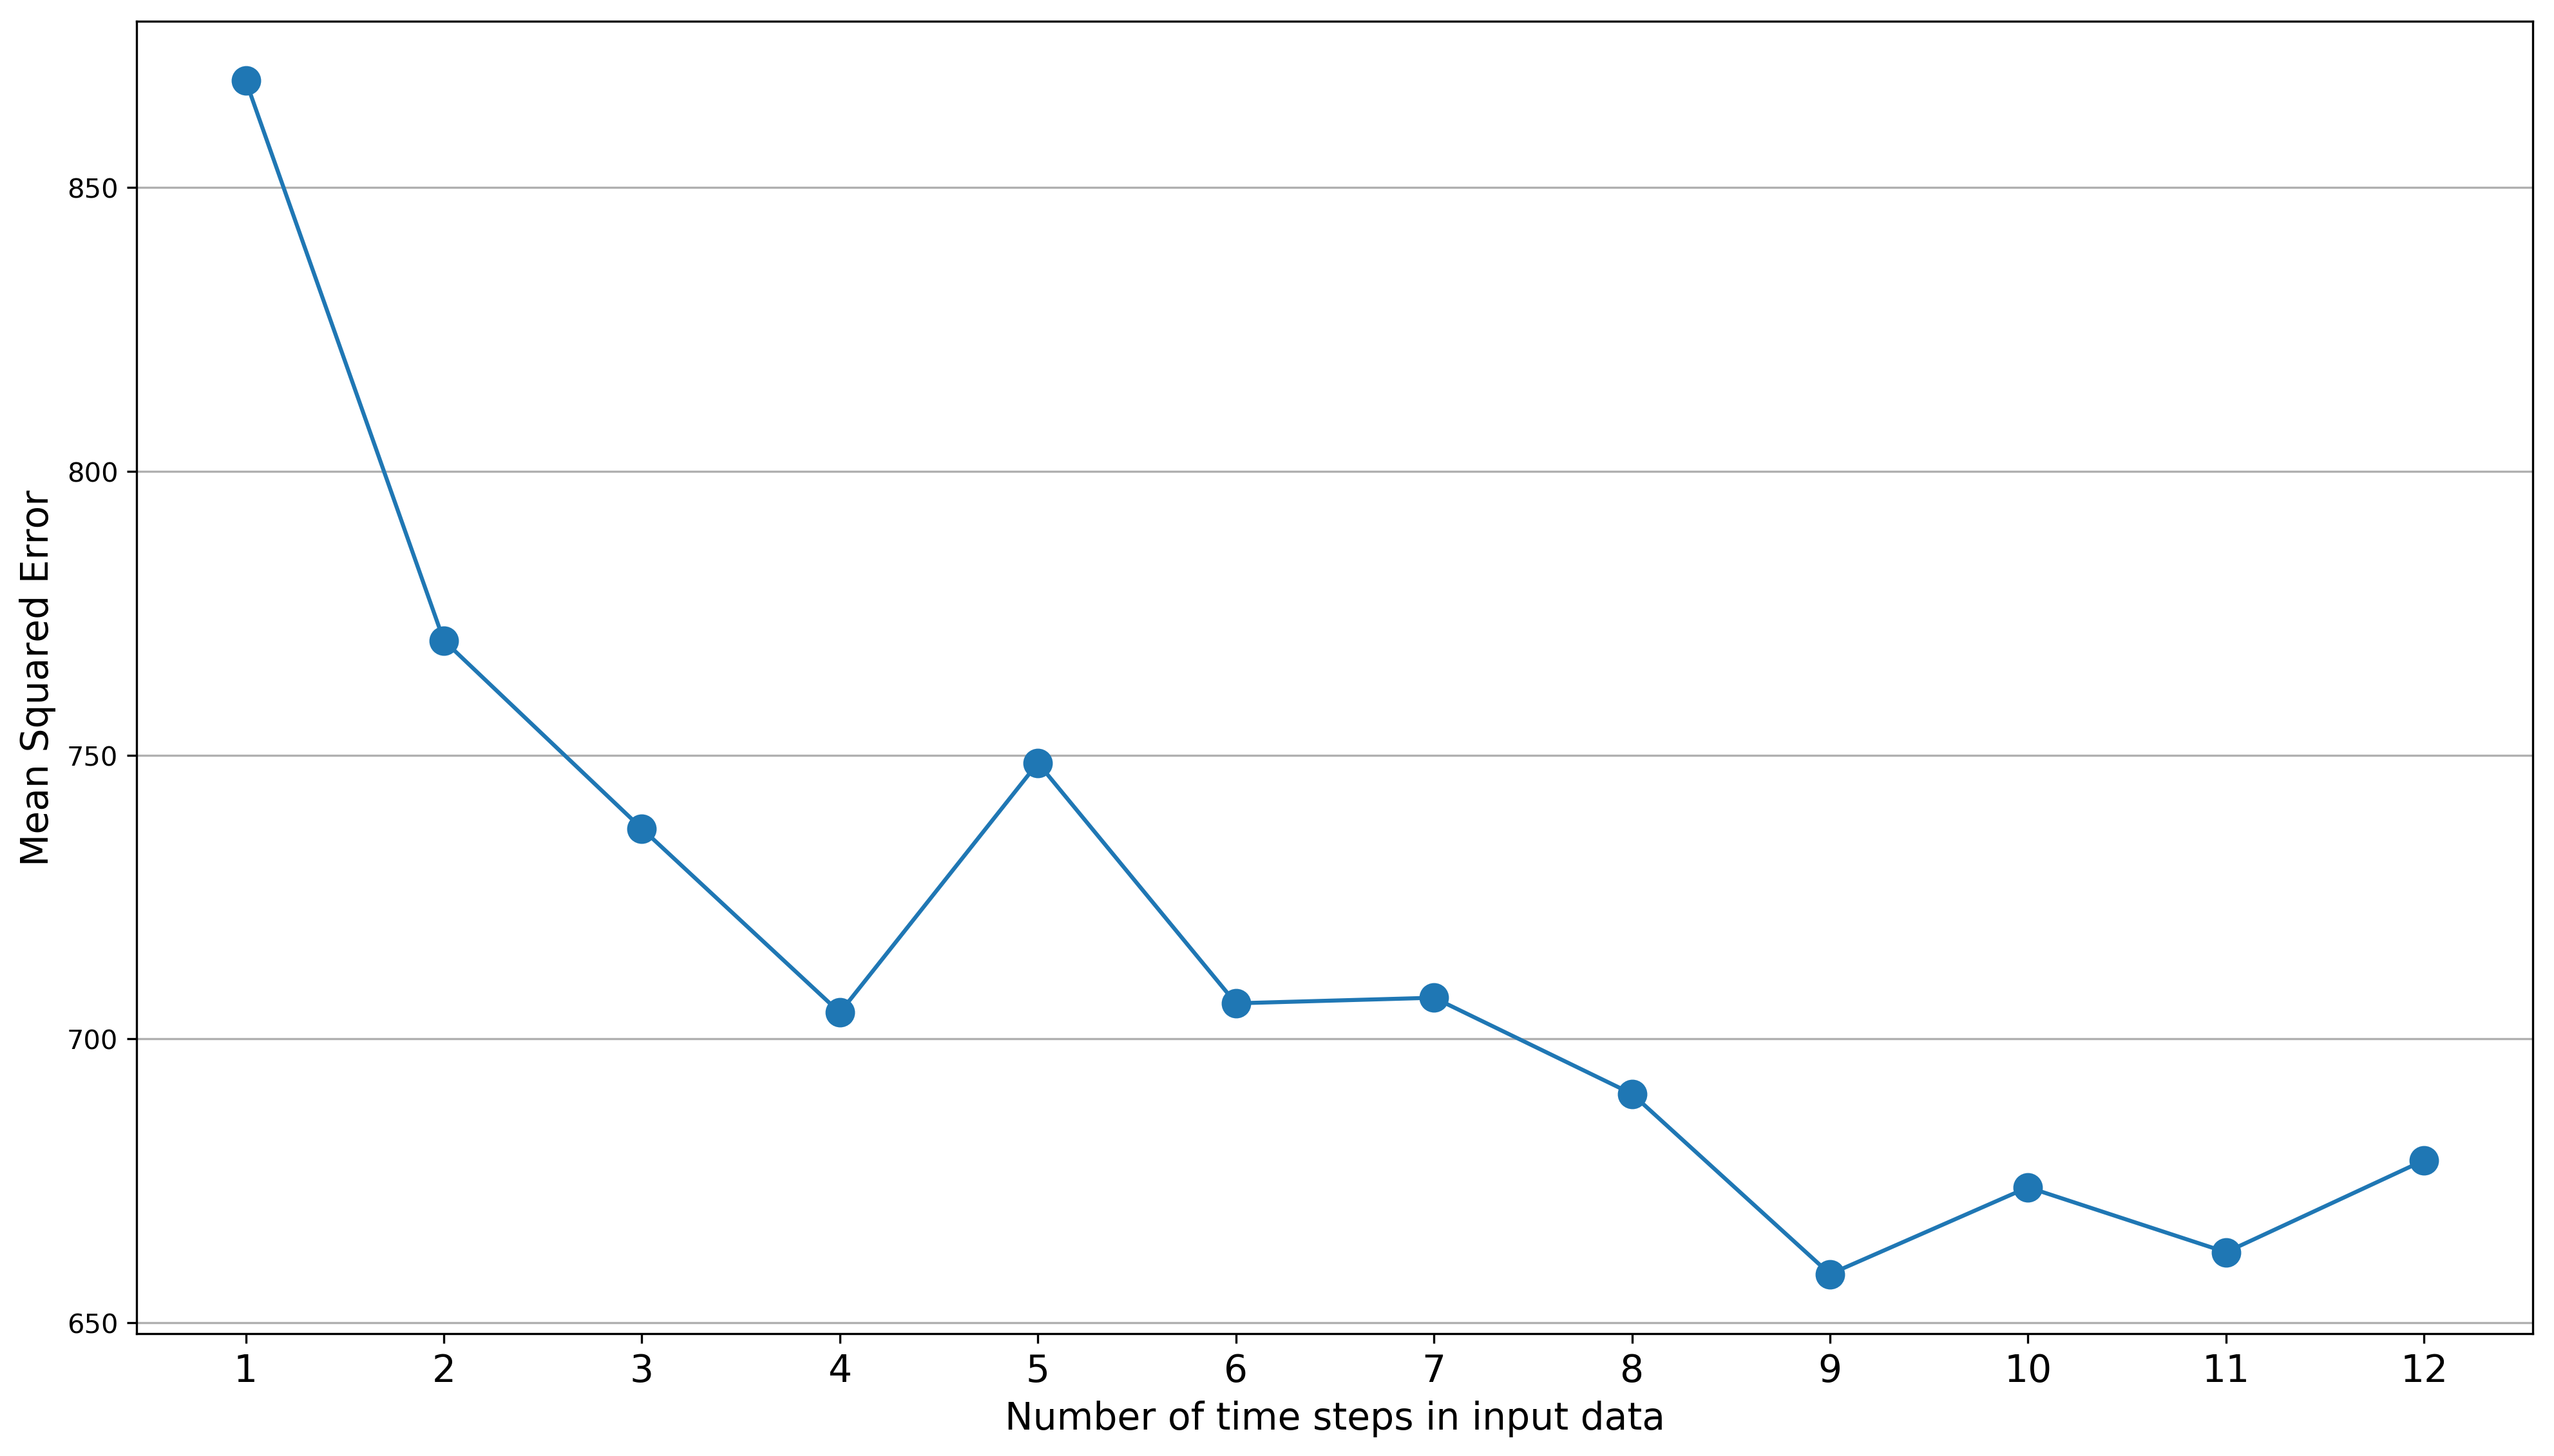
\includegraphics[width=16cm]{imgs/ts_vs_mse.png}
\caption{Influence of the number of trees in Extra Tree Regressor to overall performance. Other parameters settings are: random\_state=17, n\_estimators=65, max\_depth=35, min\_samples\_split=2, min\_samples\_leaf=1, max\_features=40, max\_leaf\_nodes=None}
\label{fig:influence_trees}
\end{figure}

\begin{figure}[h!]
\centering
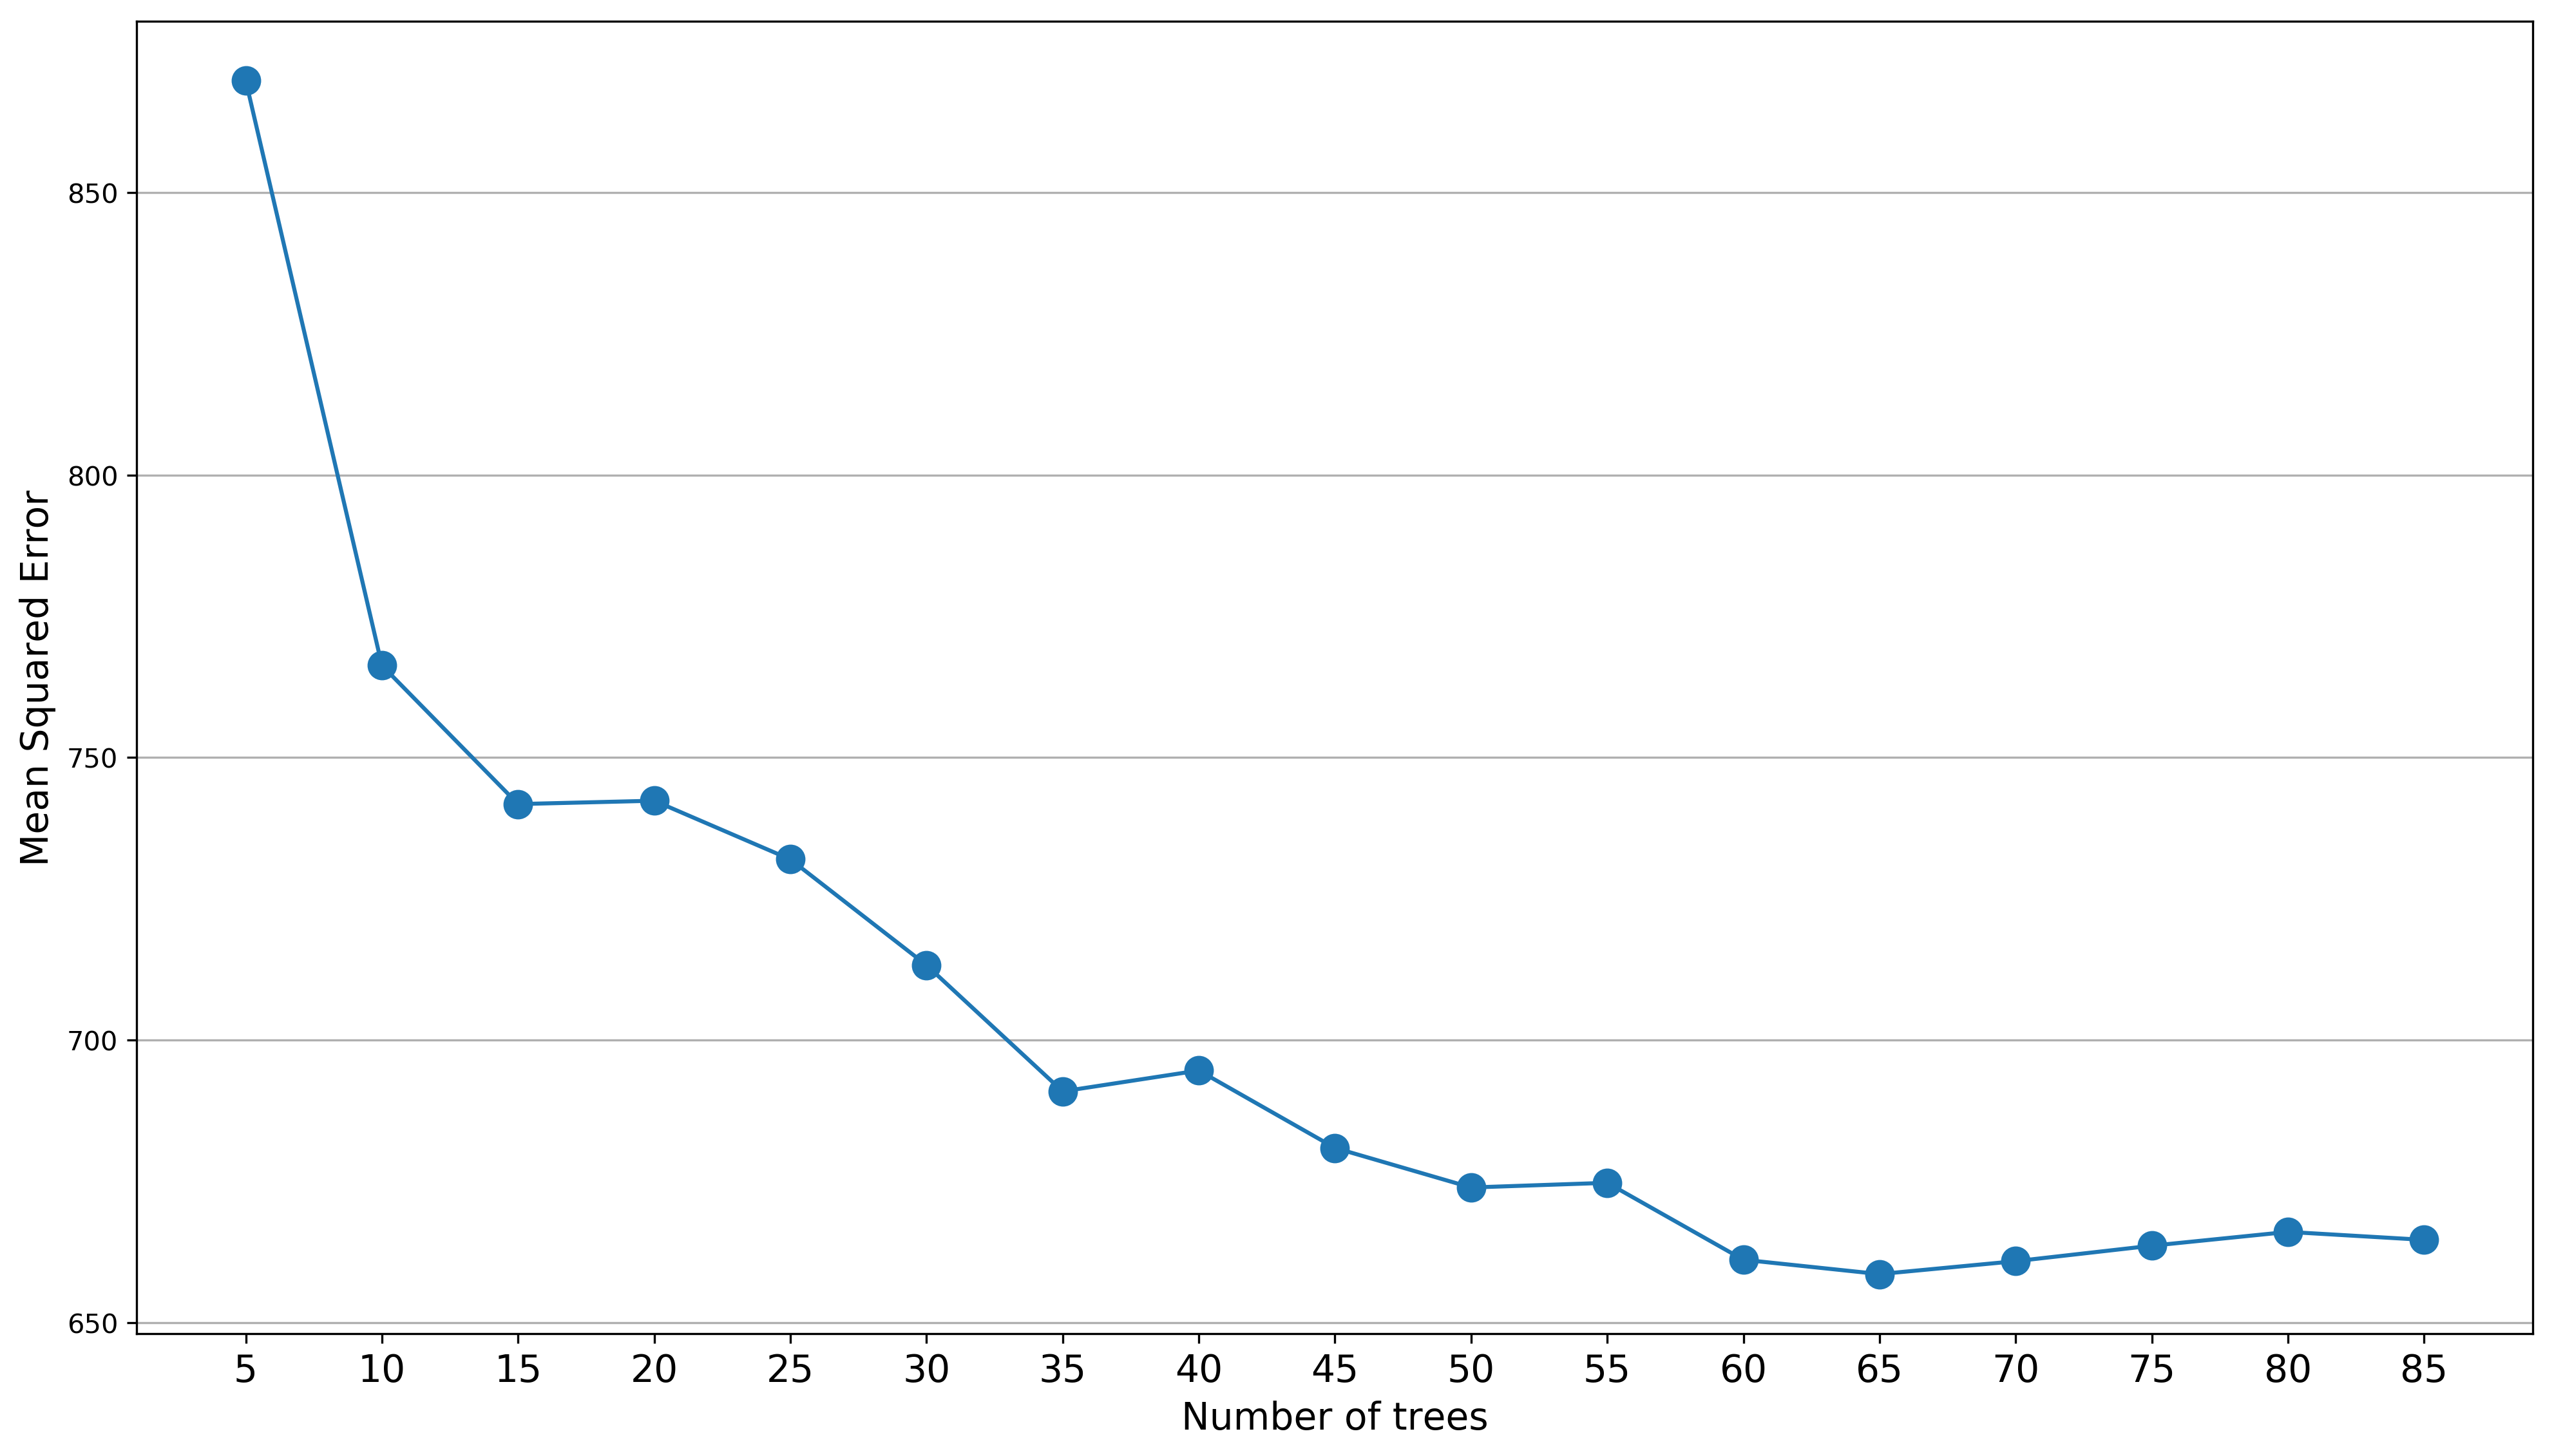
\includegraphics[width=16cm]{imgs/trees_vs_mse.png}
\caption{Influence of the number of time samples in input data of Extra Tree Regressor to overall performance. Other parameters settings are: number\_of\_input\_data\_time\_steps=9, random\_state=17, max\_depth=35, min\_samples\_split=2, min\_samples\_leaf=1, max\_features=40, max\_leaf\_nodes=None}
\label{fig:influence_ts}
\end{figure}

Best performing model overall was without doubt Extra Tree Regressor. During tuning of this were probably most interesting changes in performance influenced by number of time steps served as input and number of trees. You can see this influence on Images \ref{fig:influence_trees} and \ref{fig:influence_ts}. With the rising number of times steps used for prediction input is MSE dropping until the best performance at 9 time steps after which the error is more or less the same. More information about previous time series development definitely helps the algorithm with better predictions but at some point too much features can contain more noise for the predictor and stops being beneficial as you can see around the point of 9 time steps on Image \ref{fig:influence_ts}. Situation is almost the same with the number of trees on Image \ref{fig:influence_trees}. Here the error still drops with increasing number of trees. But for the number of trees above 65 is MSE almost the same (rising slightly) while training time and size of model rises a lot. 65 seems to be the number of trees when anything more will not influence overall performance and the prediction can no longer benefit from the randomness of extra trees. That is why number of trees 65 was chosen as the best fit for final model.


\subsection{Reflection}

\subsection{Improvement}
The biggest disappointment was definitely performance of neural network models. This is the first candidate for improvements. Different network architecture, more training data and better analysis of similar problems solved by neural networks should help with finding what went wrong and improve the performance to levels of Extra Tree Regressor or even to better results.

Another place to improve the results is usage of previous days and last week in predictions. From the data can be seen that day to day changes are usually very small and also same day in week have similar weekly attendance patters. I believe that this could be used to improve prediction even further. 

Usage of different algorithms is another possible improvement. Hidden Markov Model (HMM) or some other graphical model should be a great fit for problem like this. I spend some time trying to implement HMM without success. But I believe that HMM's could have even better results than so far best performing regressors.

\bibliographystyle{plain}
\bibliography{references}
\end{document}